
%% This style is provided exclusively for the ICSE 2012 main conference,
%% ICSE 2012 co-located events, and ICSE 2012 workshops.

%% bare_conf_ICSE12.tex
%% V1.4
%% 2012-01-21
%%

%% This is a skeleton file demonstrating the use of IEEEtran.cls
%% (requires IEEEtran.cls version 1.7 or later) with an IEEE conference paper.
%%
%% Support sites:
%% http://www.michaelshell.org/tex/ieeetran/
%% http://www.ctan.org/tex-archive/macros/latex/contrib/IEEEtran/
%% and
%% http://www.ieee.org/

%%*************************************************************************
%% Legal Notice:
%% This code is offered as-is without any warranty either expressed or
%% implied; without even the implied warranty of MERCHANTABILITY or
%% FITNESS FOR A PARTICULAR PURPOSE! 
%% User assumes all risk.
%% In no event shall IEEE or any contributor to this code be liable for
%% any damages or losses, including, but not limited to, incidental,
%% consequential, or any other damages, resulting from the use or misuse
%% of any information contained here.
%%
%% All comments are the opinions of their respective authors and are not
%% necessarily endorsed by the IEEE.
%%
%% This work is distributed under the LaTeX Project Public License (LPPL)
%% ( http://www.latex-project.org/ ) version 1.3, and may be freely used,
%% distributed and modified. A copy of the LPPL, version 1.3, is included
%% in the base LaTeX documentation of all distributions of LaTeX released
%% 2003/12/01 or later.
%% Retain all contribution notices and credits.
%% ** Modified files should be clearly indicated as such, including  **
%% ** renaming them and changing author support contact information. **
%%
%% File list of work: IEEEtran.cls, IEEEtran_HOWTO.pdf, bare_adv.tex,
%%                    bare_conf.tex, bare_jrnl.tex, bare_jrnl_compsoc.tex
%%*************************************************************************

% *** Authors should verify (and, if needed, correct) their LaTeX system  ***
% *** with the testflow diagnostic prior to trusting their LaTeX platform ***
% *** with production work. IEEE's font choices can trigger bugs that do  ***
% *** not appear when using other class files.                            ***
% The testflow support page is at:
% http://www.michaelshell.org/tex/testflow/



% Note that the a4paper option is mainly intended so that authors in
% countries using A4 can easily print to A4 and see how their papers will
% look in print - the typesetting of the document will not typically be
% affected with changes in paper size (but the bottom and side margins will).
% Use the testflow package mentioned above to verify correct handling of
% both paper sizes by the user's LaTeX system.
%
% Also note that the "draftcls" or "draftclsnofoot", not "draft", option
% should be used if it is desired that the figures are to be displayed in
% draft mode.
%
\documentclass[10pt, conference, compsocconf]{IEEEtran}
% Add the compsocconf option for Computer Society conferences.
%
% If IEEEtran.cls has not been installed into the LaTeX system files,
% manually specify the path to it like:
% \documentclass[conference]{../sty/IEEEtran}

\usepackage{graphicx,amssymb,amstext,amsmath}
\usepackage{balance}
\usepackage{hyperref}
\usepackage{multirow}


% Some very useful LaTeX packages include:
% (uncomment the ones you want to load)


% *** MISC UTILITY PACKAGES ***
%
%\usepackage{ifpdf}
% Heiko Oberdiek's ifpdf.sty is very useful if you need conditional
% compilation based on whether the output is pdf or dvi.
% usage:
% \ifpdf
%   % pdf code
% \else
%   % dvi code
% \fi
% The latest version of ifpdf.sty can be obtained from:
% http://www.ctan.org/tex-archive/macros/latex/contrib/oberdiek/
% Also, note that IEEEtran.cls V1.7 and later provides a builtin
% \ifCLASSINFOpdf conditional that works the same way.
% When switching from latex to pdflatex and vice-versa, the compiler may
% have to be run twice to clear warning/error messages.






% *** CITATION PACKAGES ***
%
%\usepackage{cite}
% cite.sty was written by Donald Arseneau
% V1.6 and later of IEEEtran pre-defines the format of the cite.sty package
% \cite{} output to follow that of IEEE. Loading the cite package will
% result in citation numbers being automatically sorted and properly
% "compressed/ranged". e.g., [1], [9], [2], [7], [5], [6] without using
% cite.sty will become [1], [2], [5]--[7], [9] using cite.sty. cite.sty's
% \cite will automatically add leading space, if needed. Use cite.sty's
% noadjust option (cite.sty V3.8 and later) if you want to turn this off.
% cite.sty is already installed on most LaTeX systems. Be sure and use
% version 4.0 (2003-05-27) and later if using hyperref.sty. cite.sty does
% not currently provide for hyperlinked citations.
% The latest version can be obtained at:
% http://www.ctan.org/tex-archive/macros/latex/contrib/cite/
% The documentation is contained in the cite.sty file itself.






% *** GRAPHICS RELATED PACKAGES ***
%
\ifCLASSINFOpdf
  % \usepackage[pdftex]{graphicx}
  % declare the path(s) where your graphic files are
  % \graphicspath{{../pdf/}{../jpeg/}}
  % and their extensions so you won't have to specify these with
  % every instance of \includegraphics
  % \DeclareGraphicsExtensions{.pdf,.jpeg,.png}
\else
  % or other class option (dvipsone, dvipdf, if not using dvips). graphicx
  % will default to the driver specified in the system graphics.cfg if no
  % driver is specified.
  % \usepackage[dvips]{graphicx}
  % declare the path(s) where your graphic files are
  % \graphicspath{{../eps/}}
  % and their extensions so you won't have to specify these with
  % every instance of \includegraphics
  % \DeclareGraphicsExtensions{.eps}
\fi
% graphicx was written by David Carlisle and Sebastian Rahtz. It is
% required if you want graphics, photos, etc. graphicx.sty is already
% installed on most LaTeX systems. The latest version and documentation can
% be obtained at: 
% http://www.ctan.org/tex-archive/macros/latex/required/graphics/
% Another good source of documentation is "Using Imported Graphics in
% LaTeX2e" by Keith Reckdahl which can be found as epslatex.ps or
% epslatex.pdf at: http://www.ctan.org/tex-archive/info/
%
% latex, and pdflatex in dvi mode, support graphics in encapsulated
% postscript (.eps) format. pdflatex in pdf mode supports graphics
% in .pdf, .jpeg, .png and .mps (metapost) formats. Users should ensure
% that all non-photo figures use a vector format (.eps, .pdf, .mps) and
% not a bitmapped formats (.jpeg, .png). IEEE frowns on bitmapped formats
% which can result in "jaggedy"/blurry rendering of lines and letters as
% well as large increases in file sizes.
%
% You can find documentation about the pdfTeX application at:
% http://www.tug.org/applications/pdftex





% *** MATH PACKAGES ***
%
%\usepackage[cmex10]{amsmath}
% A popular package from the American Mathematical Society that provides
% many useful and powerful commands for dealing with mathematics. If using
% it, be sure to load this package with the cmex10 option to ensure that
% only type 1 fonts will utilized at all point sizes. Without this option,
% it is possible that some math symbols, particularly those within
% footnotes, will be rendered in bitmap form which will result in a
% document that can not be IEEE Xplore compliant!
%
% Also, note that the amsmath package sets \interdisplaylinepenalty to 10000
% thus preventing page breaks from occurring within multiline equations. Use:
%\interdisplaylinepenalty=2500
% after loading amsmath to restore such page breaks as IEEEtran.cls normally
% does. amsmath.sty is already installed on most LaTeX systems. The latest
% version and documentation can be obtained at:
% http://www.ctan.org/tex-archive/macros/latex/required/amslatex/math/





% *** SPECIALIZED LIST PACKAGES ***
%
%\usepackage{algorithmic}
% algorithmic.sty was written by Peter Williams and Rogerio Brito.
% This package provides an algorithmic environment fo describing algorithms.
% You can use the algorithmic environment in-text or within a figure
% environment to provide for a floating algorithm. Do NOT use the algorithm
% floating environment provided by algorithm.sty (by the same authors) or
% algorithm2e.sty (by Christophe Fiorio) as IEEE does not use dedicated
% algorithm float types and packages that provide these will not provide
% correct IEEE style captions. The latest version and documentation of
% algorithmic.sty can be obtained at:
% http://www.ctan.org/tex-archive/macros/latex/contrib/algorithms/
% There is also a support site at:
% http://algorithms.berlios.de/index.html
% Also of interest may be the (relatively newer and more customizable)
% algorithmicx.sty package by Szasz Janos:
% http://www.ctan.org/tex-archive/macros/latex/contrib/algorithmicx/




% *** ALIGNMENT PACKAGES ***
%
%\usepackage{array}
% Frank Mittelbach's and David Carlisle's array.sty patches and improves
% the standard LaTeX2e array and tabular environments to provide better
% appearance and additional user controls. As the default LaTeX2e table
% generation code is lacking to the point of almost being broken with
% respect to the quality of the end results, all users are strongly
% advised to use an enhanced (at the very least that provided by array.sty)
% set of table tools. array.sty is already installed on most systems. The
% latest version and documentation can be obtained at:
% http://www.ctan.org/tex-archive/macros/latex/required/tools/


%\usepackage{mdwmath}
%\usepackage{mdwtab}
% Also highly recommended is Mark Wooding's extremely powerful MDW tools,
% especially mdwmath.sty and mdwtab.sty which are used to format equations
% and tables, respectively. The MDWtools set is already installed on most
% LaTeX systems. The lastest version and documentation is available at:
% http://www.ctan.org/tex-archive/macros/latex/contrib/mdwtools/


% IEEEtran contains the IEEEeqnarray family of commands that can be used to
% generate multiline equations as well as matrices, tables, etc., of high
% quality.


%\usepackage{eqparbox}
% Also of notable interest is Scott Pakin's eqparbox package for creating
% (automatically sized) equal width boxes - aka "natural width parboxes".
% Available at:
% http://www.ctan.org/tex-archive/macros/latex/contrib/eqparbox/





% *** SUBFIGURE PACKAGES ***
%\usepackage[tight,footnotesize]{subfigure}
% subfigure.sty was written by Steven Douglas Cochran. This package makes it
% easy to put subfigures in your figures. e.g., "Figure 1a and 1b". For IEEE
% work, it is a good idea to load it with the tight package option to reduce
% the amount of white space around the subfigures. subfigure.sty is already
% installed on most LaTeX systems. The latest version and documentation can
% be obtained at:
% http://www.ctan.org/tex-archive/obsolete/macros/latex/contrib/subfigure/
% subfigure.sty has been superceeded by subfig.sty.



%\usepackage[caption=false]{caption}
%\usepackage[font=footnotesize]{subfig}
% subfig.sty, also written by Steven Douglas Cochran, is the modern
% replacement for subfigure.sty. However, subfig.sty requires and
% automatically loads Axel Sommerfeldt's caption.sty which will override
% IEEEtran.cls handling of captions and this will result in nonIEEE style
% figure/table captions. To prevent this problem, be sure and preload
% caption.sty with its "caption=false" package option. This is will preserve
% IEEEtran.cls handing of captions. Version 1.3 (2005/06/28) and later 
% (recommended due to many improvements over 1.2) of subfig.sty supports
% the caption=false option directly:
%\usepackage[caption=false,font=footnotesize]{subfig}
%
% The latest version and documentation can be obtained at:
% http://www.ctan.org/tex-archive/macros/latex/contrib/subfig/
% The latest version and documentation of caption.sty can be obtained at:
% http://www.ctan.org/tex-archive/macros/latex/contrib/caption/




% *** FLOAT PACKAGES ***
%
%\usepackage{fixltx2e}
% fixltx2e, the successor to the earlier fix2col.sty, was written by
% Frank Mittelbach and David Carlisle. This package corrects a few problems
% in the LaTeX2e kernel, the most notable of which is that in current
% LaTeX2e releases, the ordering of single and double column floats is not
% guaranteed to be preserved. Thus, an unpatched LaTeX2e can allow a
% single column figure to be placed prior to an earlier double column
% figure. The latest version and documentation can be found at:
% http://www.ctan.org/tex-archive/macros/latex/base/



%\usepackage{stfloats}
% stfloats.sty was written by Sigitas Tolusis. This package gives LaTeX2e
% the ability to do double column floats at the bottom of the page as well
% as the top. (e.g., "\begin{figure*}[!b]" is not normally possible in
% LaTeX2e). It also provides a command:
%\fnbelowfloat
% to enable the placement of footnotes below bottom floats (the standard
% LaTeX2e kernel puts them above bottom floats). This is an invasive package
% which rewrites many portions of the LaTeX2e float routines. It may not work
% with other packages that modify the LaTeX2e float routines. The latest
% version and documentation can be obtained at:
% http://www.ctan.org/tex-archive/macros/latex/contrib/sttools/
% Documentation is contained in the stfloats.sty comments as well as in the
% presfull.pdf file. Do not use the stfloats baselinefloat ability as IEEE
% does not allow \baselineskip to stretch. Authors submitting work to the
% IEEE should note that IEEE rarely uses double column equations and
% that authors should try to avoid such use. Do not be tempted to use the
% cuted.sty or midfloat.sty packages (also by Sigitas Tolusis) as IEEE does
% not format its papers in such ways.





% *** PDF, URL AND HYPERLINK PACKAGES ***
%
%\usepackage{url}
% url.sty was written by Donald Arseneau. It provides better support for
% handling and breaking URLs. url.sty is already installed on most LaTeX
% systems. The latest version can be obtained at:
% http://www.ctan.org/tex-archive/macros/latex/contrib/misc/
% Read the url.sty source comments for usage information. Basically,
% \url{my_url_here}.





% *** Do not adjust lengths that control margins, column widths, etc. ***
% *** Do not use packages that alter fonts (such as pslatex).         ***
% There should be no need to do such things with IEEEtran.cls V1.6 and later.
% (Unless specifically asked to do so by the journal or conference you plan
% to submit to, of course. )


% correct bad hyphenation here
\hyphenation{op-tical net-works semi-conduc-tor}


\begin{document}
%
% paper title
% can use linebreaks \\ within to get better formatting as desired
\title{Fragmentation: A Comparison of Android Vendor's Bugs via Topic Analysis}


% author names and affiliations
% use a multiple column layout for up to two different
% affiliations

\author{\IEEEauthorblockN{Dan Han, Chenlei Zhang, Xiaochao Fan, Abram Hindle, Kenny Wong and Eleni Stroulia}
\IEEEauthorblockA{Department of Computing Science\\
University of Alberta \\
Edmonton, Canada\\
\{dhan3, chenlei1, xf2, hindle1, kenw, stroulia\}@cs.ualberta.ca}

}

% conference papers do not typically use \thanks and this command
% is locked out in conference mode. If really needed, such as for
% the acknowledgment of grants, issue a \IEEEoverridecommandlockouts
% after \documentclass

% for over three affiliations, or if they all won't fit within the width
% of the page, use this alternative format:
% 
%\author{\IEEEauthorblockN{Michael Shell\IEEEauthorrefmark{1},
%Homer Simpson\IEEEauthorrefmark{2},
%James Kirk\IEEEauthorrefmark{3}, 
%Montgomery Scott\IEEEauthorrefmark{3} and
%Eldon Tyrell\IEEEauthorrefmark{4}}
%\IEEEauthorblockA{\IEEEauthorrefmark{1}School of Electrical and Computer Engineering\\
%Georgia Institute of Technology,
%Atlanta, Georgia 30332--0250\\ Email: see http://www.michaelshell.org/contact.html}
%\IEEEauthorblockA{\IEEEauthorrefmark{2}Twentieth Century Fox, Springfield, USA\\
%Email: homer@thesimpsons.com}
%\IEEEauthorblockA{\IEEEauthorrefmark{3}Starfleet Academy, San Francisco, California 96678-2391\\
%Telephone: (800) 555--1212, Fax: (888) 555--1212}
%\IEEEauthorblockA{\IEEEauthorrefmark{4}Tyrell Inc., 123 Replicant Street, Los Angeles, California 90210--4321}}




% use for special paper notices
%\IEEEspecialpapernotice{(Invited Paper)}




% make the title area
\maketitle


\begin{abstract}
Android fragmentation has been a controversial topic. In this study, we investigated the fragmentation of Android by a comparison of Android vendor's bug reports via topic analysis. We mined and analyzed the Android bug reports related to two popular Android vendors, HTC and Motorola. We manually annotated bug reports with labels and applied Labeled Latent Dirichlet Allocation (Labeled-LDA) to the datasets to produce bug topics. By comparing the distribution of average relevance of top 18 bug topics over time for both vendors, we categorized the topics into three types which are \textit{Common Troubled Topics}, \textit{Common Improved Topics} and \textit{Unique Topics}. The \textit{Common Troubled Topics} show that there is no correlation between the troubled features of Android and Android evolution. The \textit{Common Improved Topics} show that some features within the same vendors have portability issues across their multiple devices. The \textit{Unique Topics} show that different vendors have specific bug topics which imply there may be the portability problem on the different vendors. Our findings can be used by Android system community, stakeholders, Android device vendors and developers to make project dashboards, process investigation and feature analysis.



\end{abstract}

\begin{IEEEkeywords}
Bug reports; Topic mining; Labeled-LDA
\end{IEEEkeywords}


% For peer review papers, you can put extra information on the cover
% page as needed:
% \ifCLASSOPTIONpeerreview
% \begin{center} \bfseries EDICS Category: 3-BBND \end{center}
% \fi
%
% For peerreview papers, this IEEEtran command inserts a page break and
% creates the second title. It will be ignored for other modes.
\IEEEpeerreviewmaketitle



\section{Introduction}
% no \IEEEPARstart

The market share of mobile phones is always changing and getting more and more competitive among various mobile device vendors\footnote{The Global Smartphone Market Landscape: \url{http://www.asymco.com/2011/11/17/the-global-smartphone-market-landscape (retrieved March, 2012)}}. The iPhone and Android phones share almost 70\% of US mobile phone market \cite{usmarket}. Compared to Apple’s closed ecosystem for iOS, in general, Android has both software fragmentation and hardware fragmentation \cite{analysis}. Android software fragmentation includes (1)multiple Android versions (2)customized device-specific Android and UI-specific Android from vendors (3) customized carrier-specific Android from vendors. Hardware fragmentation means that at any given point in time, devices based on the same Android are running on different types of hardware, related to processors, graphics processors, and screen size \cite{analysis}. The fragmentation leads to the additional testing work for Android application across multiple devices; it stops Android users experiencing some new features of Android because of the upgrading delay; and it also makes people lose confidence in Android.


Android fragmentation has been a controversial topic which swells up now and again regrading its provenance and its impacts.  However, no one can provide strong evidences to support their statements. Someone from industry performed experiments of Android on different devices, and they found that the root cause of fragmentation is the classical software engineering issues \cite{testing}.

In this study, we want to explore the fragmentation of Android by mining and analyzing Android user bug reports. We applied topic analysis on the Android bug reports. A topic of the document (e.g. bug reports, source code changes and commits) is generated by topic models which has been used to help understand software systems. There are a few topic models utilized by researchers in software engineering, e.g. Latent Dirichlet Allocation (LDA), Latent Semantic Index (LSI) and Labeled Latent Dirichlet Allocation (Labeled-LDA) \cite{Marcus04aninformation}, \cite{Asuncion:2010}, \cite{Linstead:2009}. We applied labeled-LDA \cite{labeledlda} on bug reports of different vendors and analyzed topics in bug reports. We then did the analysis on the bug topics and based on the topics analysis, we discussed what features of Android contribute much on Android fragmentation in the end. 
	
In terms of bug reports, we chose the bug reports of HTC and Motorola in this study. HTC's first Android phone was the HTC Dream manufactured in Oct. 2008. HTC has made more than thirty different Android phones since then. Motorola made their first Android phone in Oct. 2009 and has released more than twenty different Android phones since then. Their Android products have gained widespread popularity. 
 
This paper makes the following contributions:
\begin{itemize}
\item we found that some features of Android contribute to both software fragmentation and hardware fragmentation.
\end{itemize}

\begin{itemize}
\item We provided a methodology which can be used to analyze other Android branches' fragmentation.
\end{itemize}

The paper is organized as follows: Section 2 describes the background; we discuss the related work in section 3; in section 4, we introduce our methodology; we apply the analysis of topic evolution models in section 5; section 6 compares and evaluates the topic models generated by LDA and labeled-LDA;  the paper concludes with a discussion of two research questions, threats to validity, conclusion and future work in section 7, 8 and 9 correspondingly.

% You must have at least 2 lines in the paragraph with the drop letter
% (should never be an issue)

%\subsection{Subsection Heading Here}
%Subsection text here.


%\subsubsection{Subsubsection Heading Here}
%Subsubsection text here.

\section{Background}
Topic analysis, with respect to Software Control Systems (SCS) is useful in a variety of text processing applications\cite{hindle9s}. It includes two main steps: topic identification and text segmentation \cite{li2003topic}. It can be used in indexing the texts automatically to retrieve information.
With it, we can understand what the main topics and sets of associated words with these topics, and where those associated words lie within the text \cite{li2003topic}. Recent topic analysis technologies include Latent Dirichlet Allocation (LDA) and Labeled-LDA.

LDA is an unsupervised topic model to credit text documents as mixtures of latent topics, where topics correspond to key word lists presented in the corpus \cite{ldawiki}. It has been successfully used in the software engineering area for mining and retrievng informations from large text corpora.

In our research, we apply Labeled-LDA to perform topic analysis. Labeled-LDA is a supervised topic model for credit attribution in multi-labeled corpora \cite{labeledlda}. It defines a one-to-one mapping between LDA’s latent topics and tags labeled by users. In other words, labeled-LDA incorporates the multiple tags into the topics learning process and only builds topics around these tags, which is quite different from LDA. LDA, as a totally unsupervised algorithm, automatically learns a set of terms for each topic on a corpus without any constraints. To apply labeled-LDA, we utilize the Stanford Topic Modeling Toolbox (STMT) \cite{stmt}. 

%\begin{figure*}[htb]
%\centering
%\includegraphics[width=1\textwidth]{bugovertime.png}
%\caption{Number of bugs with the major version of Android for HTC and Motorola}
%\end{figure*}



\section{Related Work}
Topic models have been used to help understand software systems. Marcus et al.\cite{Marcus04aninformation} used Latent Semantic Indexing (LSI) on both source code and user queries and then identified the most relevant source code documents with similarity measurements. Asuncion et al.\cite{Asuncion:2010} applied a coherence measurement on topics learned by LDA to model the quality of bug reports. Linstead et al.\cite{Linstead:2009} performed LDA to generate traceability links for artifacts in software projects automatically. Topic modeling is also utilized by Thomas et al.\cite{Thomas:2011} to study the evolution of topics in software projects.

Compared with all these approaches, the most important difference is the topic models. They used LDA to extract topics, while we used Labeled-LDA to obtain the topics. With LDA, they prefined the number of topics and interpreted the extracted topics to get the extracted topics\cite{Asuncion:2010}. In our work, we first manually labeled bug reports with multiple labels. Then we employed labeled-LDA to get the topics. Another difference is that there is some manual work in our study to overcome the disadvantages of these unsupervised algorithms by pre-defining the number of topics and interpreting the extracted topics. 

\section{Methodology}

Our methodology is to extract bug reports, assign multiple labels to each of them and then apply labeled-LDA on the labeled data. After that we calculate the average relevance of bug reports to each label over time\cite{Hindle} and compare them between two Android vendors, HTC and Motorola. In order to compare the performance between LDA and labeled-LDA, we also apply LDA on the extracted bug reports of HTC and Motorola without our manual labels. We label all the topics generated by LDA. For each vendor, we calculate the similarity of each pair of labels from LDA and labeled-LDA to evaluate their performance.

\subsection{Generating the data}

% 1. Extract data: We converted the XML dump of bug reports into SQL
% database. We extracted all the bug reports of HTC and Motorola from
% the SQL database using regular expressions,
% e.g. '%[^0-9a-z]HTC[^0-9a-z]%' and '%[^0-9a-z]motorola[^0-9a-z]%'. We
% also removed the declined and duplicated bug reports.

% XXX: Make sure that the reason behind HTC and Motorola were already
% made clear by this point

Our first step was to extract the Android bug reports and then find
those bug reports relevant to HTC and Motorola
We use the Android bug reports provided by the MSR Mining
Challenge~\cite{MSRChallenge2012}
and parse store the bug reports, described as XML data, into a
database using SQL
Server. 

Then we selected bug reports that identified themselves as being
relevant to HTC or Motorola through a mention of the words HTC or
Motorola in the title text, description text of the bug report.  
We used regular expressions to extract these relevant bug reports (e.g.,$'\%[\hat{ }0-9a-z]htc[ \hat{ }0-9a-z]\%'$ and $'\%[ \hat{ }0-9a-z]motorola[ \hat{ }0-9a-z]\%'$).
%`\texttt{[\^0-9a-z]HTC[\^0-9a-z]}' and
%`\texttt{[\^0-9a-z]motorola[\^0-9a-z]}').
% Using regexes, we extract bug reports highly related to
% Android phones of HTC and Motorola respectively. 
% We use the title,
% opened date and description in each bug report. 
% XXX: What does declined mean: There is a status field in the bug repo. "Declined" is a bug status which means bug reports are not accepted by the bug repo, e.g. the bug reports might not be related to Android devices.
We then removed all the declined and duplicate bug reports, leaving us
with 1503 HTC bug reports and 1058 Motorola bug reports.

\begin{table}[!t]
\renewcommand{\arraystretch}{1.3}
% if using array.sty, it might be a good idea to tweak the value of
% \extrarowheight as needed to properly center the text within the cells
\caption{Manual labels from bug reports of HTC and Motorola.}
\label{selected1}
\centering
\begin{tabular}{|c||l|}
\hline
Vendor & Label\\
\hline
HTC & sms\//mms calling email contact video time network system\\ 
  & android\_market display browser bluetooth audio memory input\\
  & notification image SIM\_card setting layout app upgrade\\
  & wifi google\_map keyboard calendar alarm language car search\\
  & dialing USB touchscreen CPU gtalk voicedialing signal\\
  & google\_voice ringtone google\_navigation location font\\
  & google\_earth battery google\_translate twitter date VPN radio\\
  & picassa video\_call rSAP region screen\_shot download\\
  & IPV6 SD\_card storage 3G proxy compass lock calculator\\
  & synchronize  voicemail  voice\_recognition facebook  flash\\
  & google\_latitude  GPS camera youtube\\
\hline
Motorola & calling network setting gtalk calendar signal contact\\
    & android\_market input camera image app wifi keyboard system\\
    & layout sms\//mms bluetooth display browser email notification\\
& alarm audio multimedia\_dock car SD\_card screen text lock\\
& voicedialing battery upgrade dialing ringtone volume GPS\\
& video time swype search exchange headset synchronize USB\\
& facebook google\_wave download youtube uploadcalculator\\
& monkey flash VPN touchscreen vibrate CPU\\
\hline
\end{tabular}
\end{table}


\subsection{Research Features as Potential Labels}

% 2. Where are the labels coming from: Before labeling all the bug
% reports, we studied the Android operating system to get the features
% of Android phones
% [http://en.wikipedia.org/wiki/Android_operating_system] and popular
% applications in Android Market
% [https://play.google.com/store/apps]. We also studied the hardware
% components of HTC and Motorola
% [http://en.wikipedia.org/wiki/Comparison_of_Android_devices]. The
% labels are based on these three aspects of Android phones.

In order to investigate fragmentation from a feature-oriented
perspective we decided we were going to label the bug reports by
relevant features in order to look for feature-relevant bug reports
for each manufacturer.
To help seed the possible feature-oriented labels we 
studied summary texts about the Android Operating
System~\footnote{Android Operating System summary:
\url{http://en.wikipedia.org/wiki/Android_operating_system} (retrieved
March, 2012)}, 
popular apps within the Android Market~\footnote{Android Market:
  \url{https://play.google.com/store/apps} (retrieved March, 2012)}.
As well we studied hardware comparisons of the popular Android handsets of 
 of HTC and Motorola~\footnote{Android Comparison:
  \url{http://en.wikipedia.org/wiki/Comparison_of_Android_devices}
  (retrieved March, 2012)}.

\subsection{Developing Labels}
%Multi-labeling}


Once we became familiar with the Android operating system and Android
ecosystem we needed to agree and train ourselves to consistently label
Android bug reports to study vendor relevant fragmentation of bug reports.

% 3. Label the bug reports: Zhang and Fan labeled 248 HTC bug reports in
% 2009 separately and then compared the results by each bug to ensure
% the same interpretation of the labels from last step. Then Zhang and
% Fan labeled the rest of the bug reports separately.

%XXX we need a cite
Following a grounded theory-like coding approach, similar to the
approach taken in by Hindle et al.~\cite{Hindle2011}, authors Zhang
and Fan selected a set of HTC 248 bug reports to label
separately. 

To label a bug report, the annotator (Zhang or Fan) reads the bug
report text, both the title and the description, and  then based on their
personal interpretation they related that bug report to the relevant
features. This means that one bug report can receive multiple labels
if it is relevant to multiple identified features. Labels were created
as necessary, if a label regarding a feature did not already exist, it
was created.
These labels 
consisted of the features and applications on an Android mobile
phone, such as SMS/MMS, browser and Wi-Fi or the components of the
handsets mentioned in the bug reports, such as GPS, screen and
keyboard.


To ensure consistency and agreement in labelling the authors executed a training
methodology. This methodology also ensured a synchronization of labels.
Each author, Zhang and Fan, separately labeled each of these 248 bug reports, 
with labels inspired by the previous research on Android
features. 
After Zhang and Fan labeled these 248 bug reports seperately, the
labels were compared and the authors discussed label agreement and
disagreement in order to train themselves to consistently label bug
report.
To help the comparison each author’s labeled data was used as input to
 STMT's implementation of Labeled-LDA which produced a set of topics.
The topics and their relevant bug reports were compared to ensure
consistent interpretation of the bug reports and their labels.



%First, two of us (Zhang and Fan) separately tag the HTC 248 bug
%reports in 2009 with the multiple labels. 
% Then we train each author’s labeled data with STMT. 
% By comparing each set of trained topics in the results and returning
% to the bug reports, we check to ensure the same interpretation of each
% bug when labeling. 
% Then we come up with the same labeling rules to process the data. 

\subsection{Labelling the HTC and Motorola Bug Reports}

Once the labelling rules were agreed upon each author (Zhang and Fan)
seperately labeled HTC and Motorola bug reports, taking over 60 man
hours of manual labelling effort.
%After this, we tag the rest of bug reports separately for both HTC and
%Motorola. 
Using the previously stated labelling methodology, labels were created as necessary.
%When there is a bug report that cannot be tagged by the labels we
%already have, we would create a new label together based on our
%definition of labels, i.e. the functionalities and applications on an
%Android mobile phone or the components of the handsets. 
For example, the label ``calculator'' was created in order to label
bug reports that occurred later that were relevant to this feature as
were several bug reports regarding the correctness of the
calculator's results. 
% So we added it to our labels. 
%The manual labelling took approximately 30 hours per person. 


1304 HTC and 985 Motorola bug reports were labeled with multiple
labels, leaving 199 and 73 bug reports that cannot be clearly labeled.
In total, there are 72 labels for HTC and 57 labels for Motorola.
Table \ref{selected1} lists all the manual labels from bug reports of HTC
and Motorola.

% XXX TODO labeled-LDA to Labeled-LDA
\subsection{Applying Labeled-LDA}


% 4. Apply labeled-LDA:We applied the Labeled-LDA tool, Stanford Topic
% Modeling Toobox [http://nlp.stanford.edu/software/tmt/tmt-0.4/], to
% get the topic-document distribution on our labeled bug reports.

% 5. Calculate the average relevance of each label: The average
% relevance over time of each label is calculated for each vendor. For
% each label the average relevance in one month is the the sum of bug
% reports' relevance divided by the number of bug reports in this
% month. The plot of the average relevance of each label between HTC
% and Motorola is based on this calculation.


Once the bug reports were labeled we wanted to extract the topics
associated with the labels. First we had to preprocess the bug reports 
in order to apply Labeled-LDA to the labeled bug reports. 
We convert the title and description of each bug report to lowercase,
tokenize and filter the words to remove stop words (words that are less than 3 characters and
common English stop words such as ``all'', ``about'', ``the'',
``that'' and ``were'' ), and then produce word counts/distribution per
each HTC bug report and each Motorola bug report.

Separately, we applied Labeled-LDA to these preprocessed HTC bug reports and Motrola bug reports.
%We then supplied Labelled-LDA with these word distributions of the bug reports.
Labeled-LDA then outputs the topic, a word distribution, associated
with our label, as well as a document-topic matrix which links our
labels to the documents in the each bug report corpus (HTC and
Motorola).
%By applying labeled-LDA to the bug reports of HTC and Motorola
%separately, we have the word distribution of each label and a matrix
%that provides the relationship between bug reports and the labels. 

The topic analysis is based on these results. 
In order to visualize the association of a label (an extracted
Labeled-LDA topic) to bug reports over time, we grouped the 
%In order to investigate the trend of each label by time, 
we grouped
all the bug reports by month from 2009 to 2011 based on their open
date for each of the two vendors. 
For each label, we computed the average relevance values of bug
reports to this label in each month. 
The average relevance value of a label \begin{math} \l_i \end{math} in month \begin{math} m_j \end{math} is the sum of all the relevance values of this label over all bug reports in this month divided by the number of bug reports in this month,
\begin{equation}
A(\l_i,m_j) = \frac{\sum_{\substack{k=1}}^{|m_j|}r(\l_i,d_k)}{|m_j|}
\label{equation1}
\end{equation}
where $r(\l_i,d_k)$ is the relevance value of label $\l_i$ to bug
report $d_k$, $|m_j|$ is the number of bug reports in this month. We generated a distribution of average relevance among three years for each label, showed in Figure\ref{commontopic}, Figure \ref{fixtopic}, Figure \ref{uniquehtc} and Figure \ref{uniquemoto}.

% XXX mention the topics
% XXX VVV what is this stuff?
%This metric is to sum all the relevance values. 
% Finally we generated a distribution of relevance among 36 months for each label.

\subsection{Applying LDA}

% 6. Apply LDA: We applied LDA on HTC and Motorola bug reports. We
% tried a set of number of topics for both vendors and in each case we
% tried to label all the topics generated by LDA based on the manual
% labels.

% 7. Choose the number of topics in LDA: We chose the number of topics
% in LDA based the rules that the topics are distinct enough from each
% other, have no repetition and can be well interpreted by us (i.e. we
% can use the manual labels to tag them).


In order to compare the performance between LDA and Labeled-LDA in
order to see if Labeled-LDA is worth the effort, 
we applied LDA to the extracted the same bug reports of HTC and Motorola
but without our manual labels. 
We used the same preprocessing method used on the bug-reports used in
the Labeled-LDA analysis.

Applying LDA had one complication, LDA requires an input, $n$ that
determines the number of topics that LDA is supposed to extract. If
$n$ is too large, the topics tend to repeat themselves and tend to
represent similar issues. If $n$ is too small, the topics tend to
be cluttered and lack a coherent topic. This can interpreted manually
by reading the topics and evaluating the top 10 or 20 words associated
with a topic.
To choose the number of topics $n$, we ran LDA using multiple values
of $n$ that included: 10, 15, 20, 25, 30, 35, 40, 45, 50, 55, 60, 65
and 70 on the bug reports of HTC. 
Three of the authors (Han, Zhang and Fan) evaluated the word distribution of each topic
together in each case. 
We determined if topics were distinct enough based on labeling. Given
our previous manual labels that were used by Labeled-LDA we tried to label these LDA topics
with those labels. If we repeated too much, or too many labels were
clustered around a topic, we considered that choice of $n$ to be unfit.
The authors chose the $n = 35$, as the topics generated by LDA
were distinct enough from each other, had few repetitions and could be
interpreted well by the authors based on their own judgment.
Other researchers had some similar results
\cite{Thomas:2011,Hindle2011,Hindle}. 

We applied the same process to the bug reports of Motorola and we chose
the number of topics to be $n = 30$. 
As described for the HTC bug reports, we also labeled each topics
generated by LDA with our manual labels.
Three of the authors annotated the topics together and it took two
hours in total to finish all the labeling work. 
Table \ref{seleted2} lists a few selected topics from LDA with manual labels.


\subsection{Comparing the Effort to Use LDA and Labeled-LDA}

% 8. Comparison of LDA and labeled-LDA: For each pair of topics in LDA
% and labeled-LDA, we computed the their similarity based on the
% topic-document distribution. That is the Jaccard similarity of the two
% sets. One is from LDA and the other one is from labeled-LDA. Each set
% is the bug reports that have relevance to that label. We chose several
% thresholds on the relevance. That is if the relevance is under the
% threshold, this bug report is not related to that label. At last we
% chose threshold to be 0.2 the mean of the similarities is the
% biggest. 

In order to determine if LDA would generate the similar results to
Labeled-LDA we had to compare the results.
% Thus nce LDA and Labelled-LDA were applied to the bug reports of HTC and
% Motorola we had to compare the topics that were extracted.
Both LDA and labeled-LDA produce matrices of
 the relationship between bug reports of two vendors and the
label or topics. 
That is if the topics generated by LDA that were labeled as the same
ones in labeled-LDA would be related to similar bug reports.

We determined topic similarity by comparing the sets of documents
relevant to a LDA topic and those relevant to a Labeled-LDA
topic. Because the LDA topic might be different from the Labeled-LDA
topic we did pair-wise similarity comparisons.

We applied the Jaccard similarity coefficient to compute the
similarity between each topic in LDA and each label in labeled-LDA. 
That is, the Jaccard similarity coefficient between label A in LDA and
label B in labeled-LDA is the ratio of the intersection of bug reports
related to label A and label B to the union of the bug reports related
to label A and label B,
\begin{equation}
sim(A,B) = \frac{\phi(A,d)\bigcap\phi(B,d)}{\phi(A,d)\bigcup\phi(B,d)}
\end{equation}
where the $\phi(A,d)$ is the set of bug reports that has relevance
values to label A and $d$ is a set of all the bug reports in each
vendor.

%XXX I still don't understand where 0.2 comes from
% under the threshold of 0.2 we computed the similarities which had the biggest mean value.
The topic-document matrix often contains quiet noise and weak
relationships between topics and documents, thus it is necessary to
provide a threshold of document relevance to determine if a document
is relevant to a topic or not.
We used several thresholds (0.01, 0.05, 0.1, 0.2, 0.3, 0.4 and 0.5) on
the relevance value of a bug report to a label in LDA when generating
the Jaccard similarity coefficients. We eventually chose $0.2$ as the similarities had the biggest mean value.
We plotted these pairwise tests in order to explore the match between
LDA and Labeled-LDA.

Then we counted the number of bug reports that are related to labels which are both shared by LDA and Labeled-LDA in HTC and Motorola. We applied the Chi-squared test on the two sets of distribution to study if each of the two distributions match.


\begin{table}[!t]
\renewcommand{\arraystretch}{1.3}
% if using array.sty, it might be a good idea to tweak the value of
% \extrarowheight as needed to properly center the text within the cells
\caption{Selected topics from LDA with manual labels. Word lists are inferred by LDA.}
\label{seleted2}
\centering
\begin{tabular}{|c||c||l|}
\hline
Vendor & Label & Top 10 terms\\
\hline
HTC & sms\//mms &sms, message, text, sent, send, conversation, \\
            && received, reply, time, number \\ \cline{2-3}
  & email & Email, mail, gmail, app. Inbox, send, emails, \\
            &&message, client, read \\ \cline{2-3}
  & browser&browser, page, web, http, open, website, \\
            &&webview, click, url, load\\
\hline
Motorola & wifi &connect, xoom, hotspot, netbook, wifi, ssid, \\
           &&radio, connection, feature, model\\ \cline{2-3}
    &calendar& calendar, event, sync, appointment, date, google, \\
           &&time, droid, day, change \\ \cline{2-3}
    &contact & contact, google, number, address, list, facebook, \\
           &&droid, account, sync, separate \\
\hline
\end{tabular}
\end{table}


\section{Topic Mining and Analysis}

In order to investigate fragmentation within Android, we mined the bug reports of Android and analyzed the result from both quantitative and qualitative aspects.

We started by exploring the distribution of number of bug reports for HTC and Motorola. Then we compared and discussed the distribution of average relevance for each topic over time for both vendors.

%\begin{figure}[!htb]
%\centering
%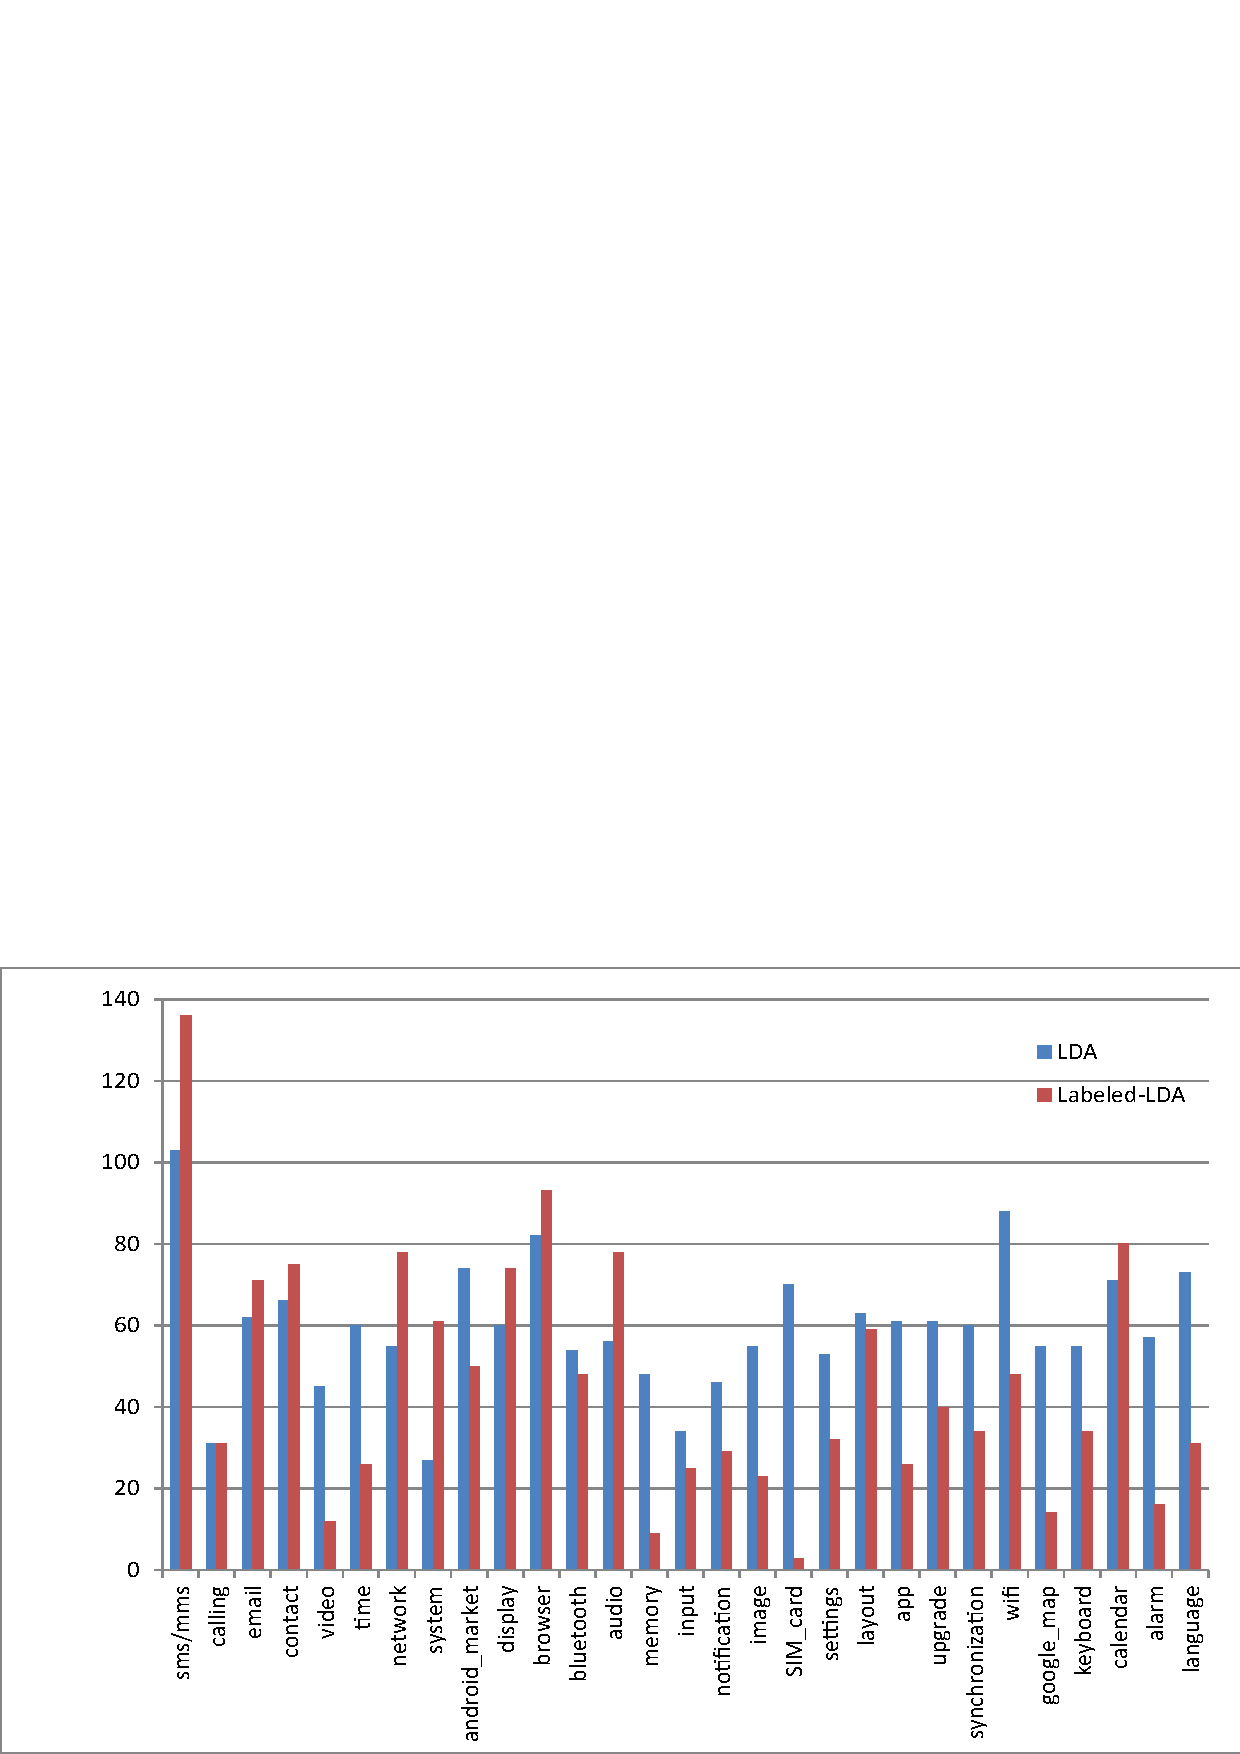
\includegraphics[width=0.4\textwidth]{htcldallda.png}
%\caption{Comparison of number of bug reports related to the same labels from LDA and labeled-LDA in HTC. The X axis is the same labels from LDA and labeled-LDA and the Y axis is the number of bug reports.}
%\end{figure}
%
%\begin{figure}[!htb]
%\centering
%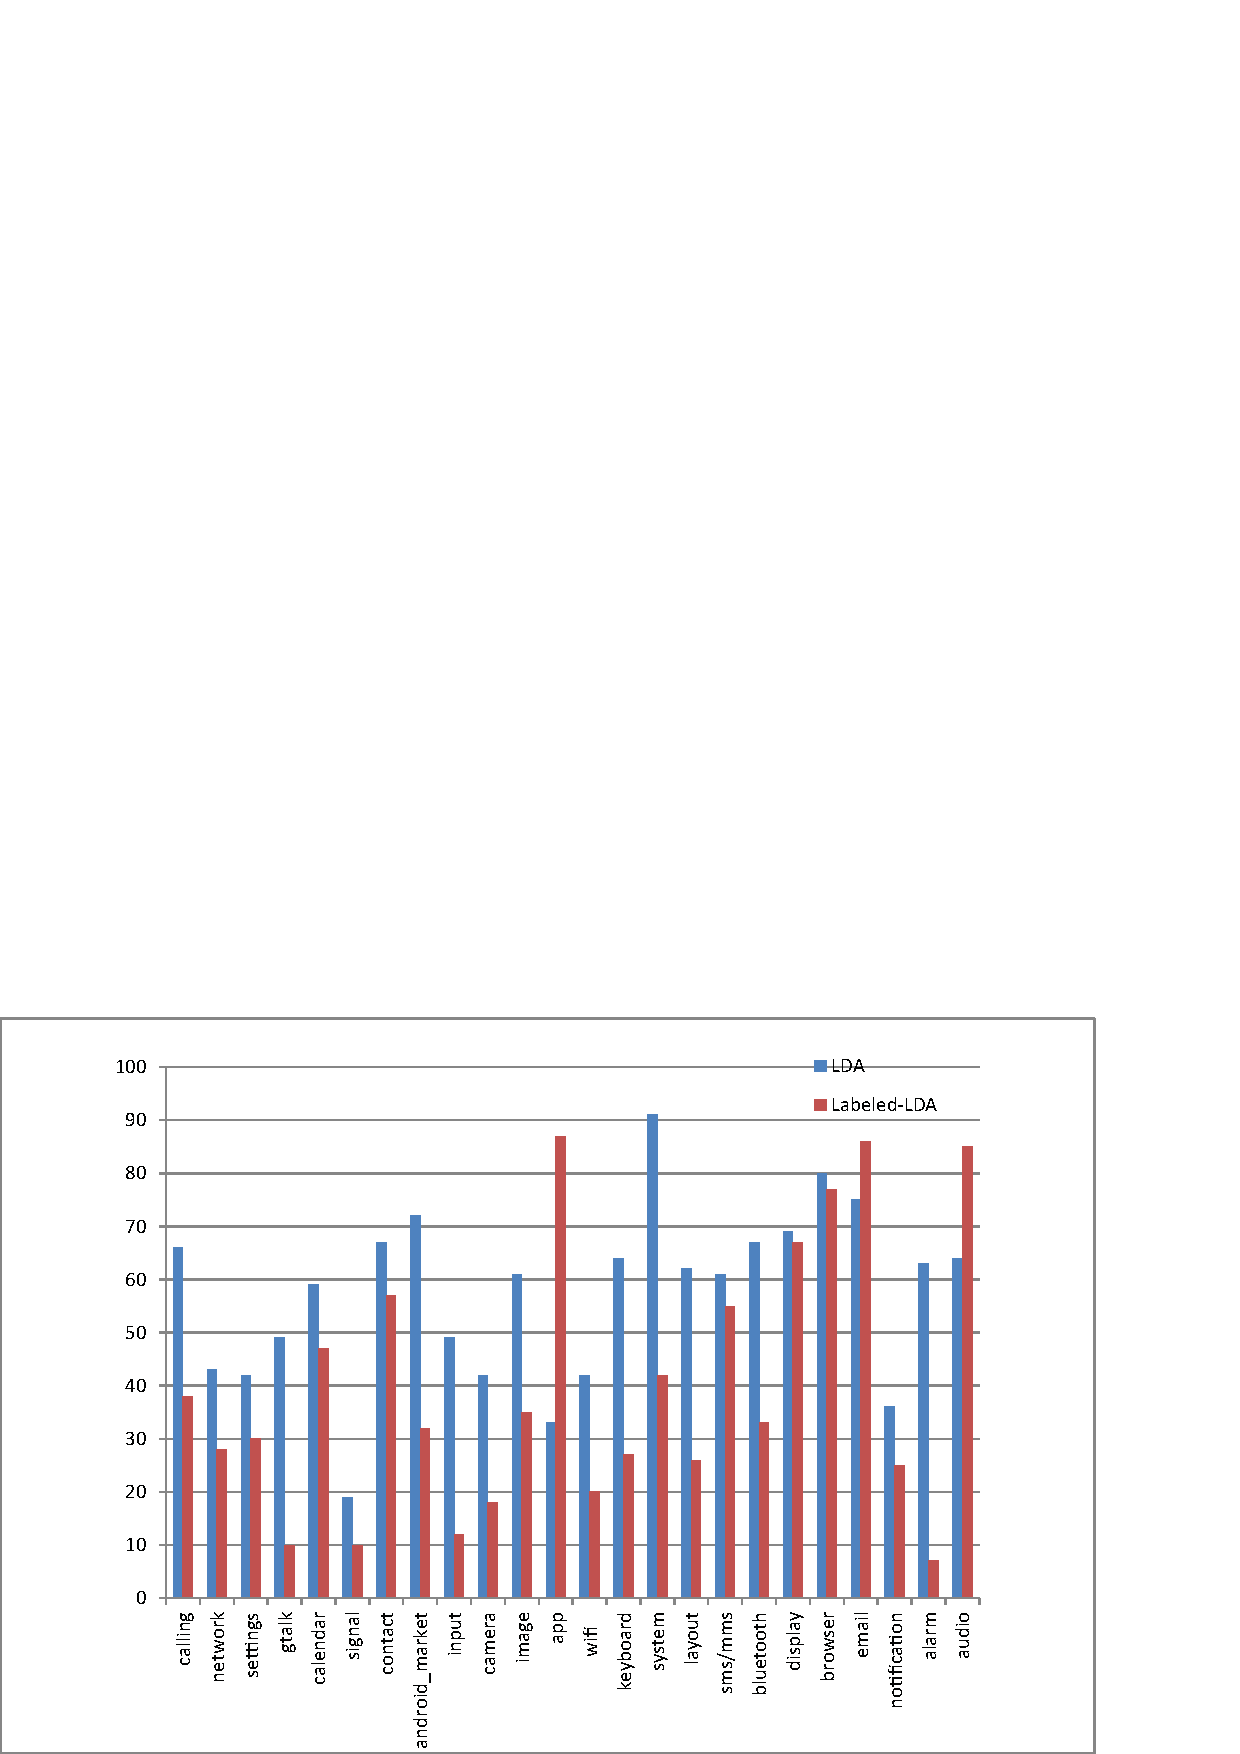
\includegraphics[width=0.4\textwidth]{motoldallda.png}
%\caption{Comparison of number of bug reports related to the same labels from LDA and labeled-LDA in Motorola. The X axis is the same labels from LDA and labeled-LDA and the Y axis is the number of bug reports.}
%\end{figure}
%
%\begin{figure}[htb]
%\centering
%\includegraphics[width=0.4\textwidth]{htcratiosim.png}
%\caption{The comparison of ratio and similarity in HTC. The result of the smaller number of bug reports related to this label in LDA or labeled-LDA divided by the larger one is the ratio of this label. The X axis is the same labels from LDA and labeled-LDA.}
%\end{figure}
%
%\begin{figure}[htb]
%\centering
%\includegraphics[width=0.4\textwidth]{motoratiosim.png}
%\caption{The comparison of ratio and similarity in Motorola. The result of the smaller number of bug reports related to this label in LDA or labeled-LDA divided by the larger one is the ratio of this label. The X axis is the same labels from LDA and labeled-LDA.}
%\end{figure}

\begin{figure*}[htb]
\centering
\includegraphics[width=1\textwidth]{bugovertime.png}
\caption{Number of bug reports with the major version of Android for HTC and Motorola}
\label{bugovertime}
\end{figure*}

\subsection{Overview of bug reports in HTC and Motorola}

We grouped the bug reports monthly based on their opened date and counted the total number of bug reports in each month for two vendors. Figure \ref{bugovertime} depicts a comparison of the number of bug reports for HTC and Motorola.

From Figure \ref{bugovertime}, we can observe that the first HTC bug report was opened in January, 2009, and the first Motorola bug report was opened in October, 2009. According to the brief history of Android devices survey \cite{historyofandroid}, HTC released the first Android device in October, 2008, while Motorola released its first device in October, 2009. The first bug reports of both vendors are in order of the first device released by them. There is a strong time correlation between the first opened bug report and the first released Android device of both vendors.

In addition, we can see, in Figure \ref{bugovertime}, the first spike for HTC happened in September, 2010, and for Motorola it happened in December, 2009. By reading the bug reports, we found that the spike of HTC was caused by the fact that many people upgraded their devices from Android 2.1 to Android 2.2 at that time, and some functions did not work well after upgrading. For example, users could not send message after the upgrading. The spike of Motorola was mainly resulted from the upgrading from Android 2.0 to Android 2.0.1. This suggests that the increasing of the number of bug reports is more relevant to Android version than hardware platform.
% xxx You didn't compare the hardware platforms. How can you have this conclision?


\subsection{Topics Analysis of HTC and Motorola}

As shown in Table \ref{selected1} we extracted 72 topics for HTC and 57 topics for Motorola with Labeled-LDA.

Based on Equation \ref{equation1} each topic has a distribution of average relevance over time. We categorized the topics into three types based by comparing each topic's distribution in both vendors. They are \textit{Common Troubled Topics}, \textit{Common Improved Topics}, and \textit{Unique Topics}. 
The \textit{Common Troubled Topics} mean that the distribution of the average relevance of the topics have fluctuations all the time for both HTC and Motorola. The \textit{Common Improved Topics} mean that the distribution of the average relevance of topics turn to be flat over time after several fluctuations for HTC and Motorola. The \textit{Unique Topics} mean that the distribution of average relevance of topics have significant differences between HTC and Motorola.

A representative subset of top 18 topics, which are obtained by
sorting the number of related bug reports for HTC and Motorola
respectively, is given in Table \ref{topicslist}.
Each topic is associated with top 15 terms generated by Labeled-LDA for
both HTC and Motorola. 
%These topics are associated with 85\% bugs of HTC, and 83\% bugs of Motorola. 
As mentioned before, the label column in Table \ref{topicslist} represents the features of Android. %Please refer to the resarch features as potential labels to have a better understanding of all the labels.

\begin{figure*}[htb]
\centering
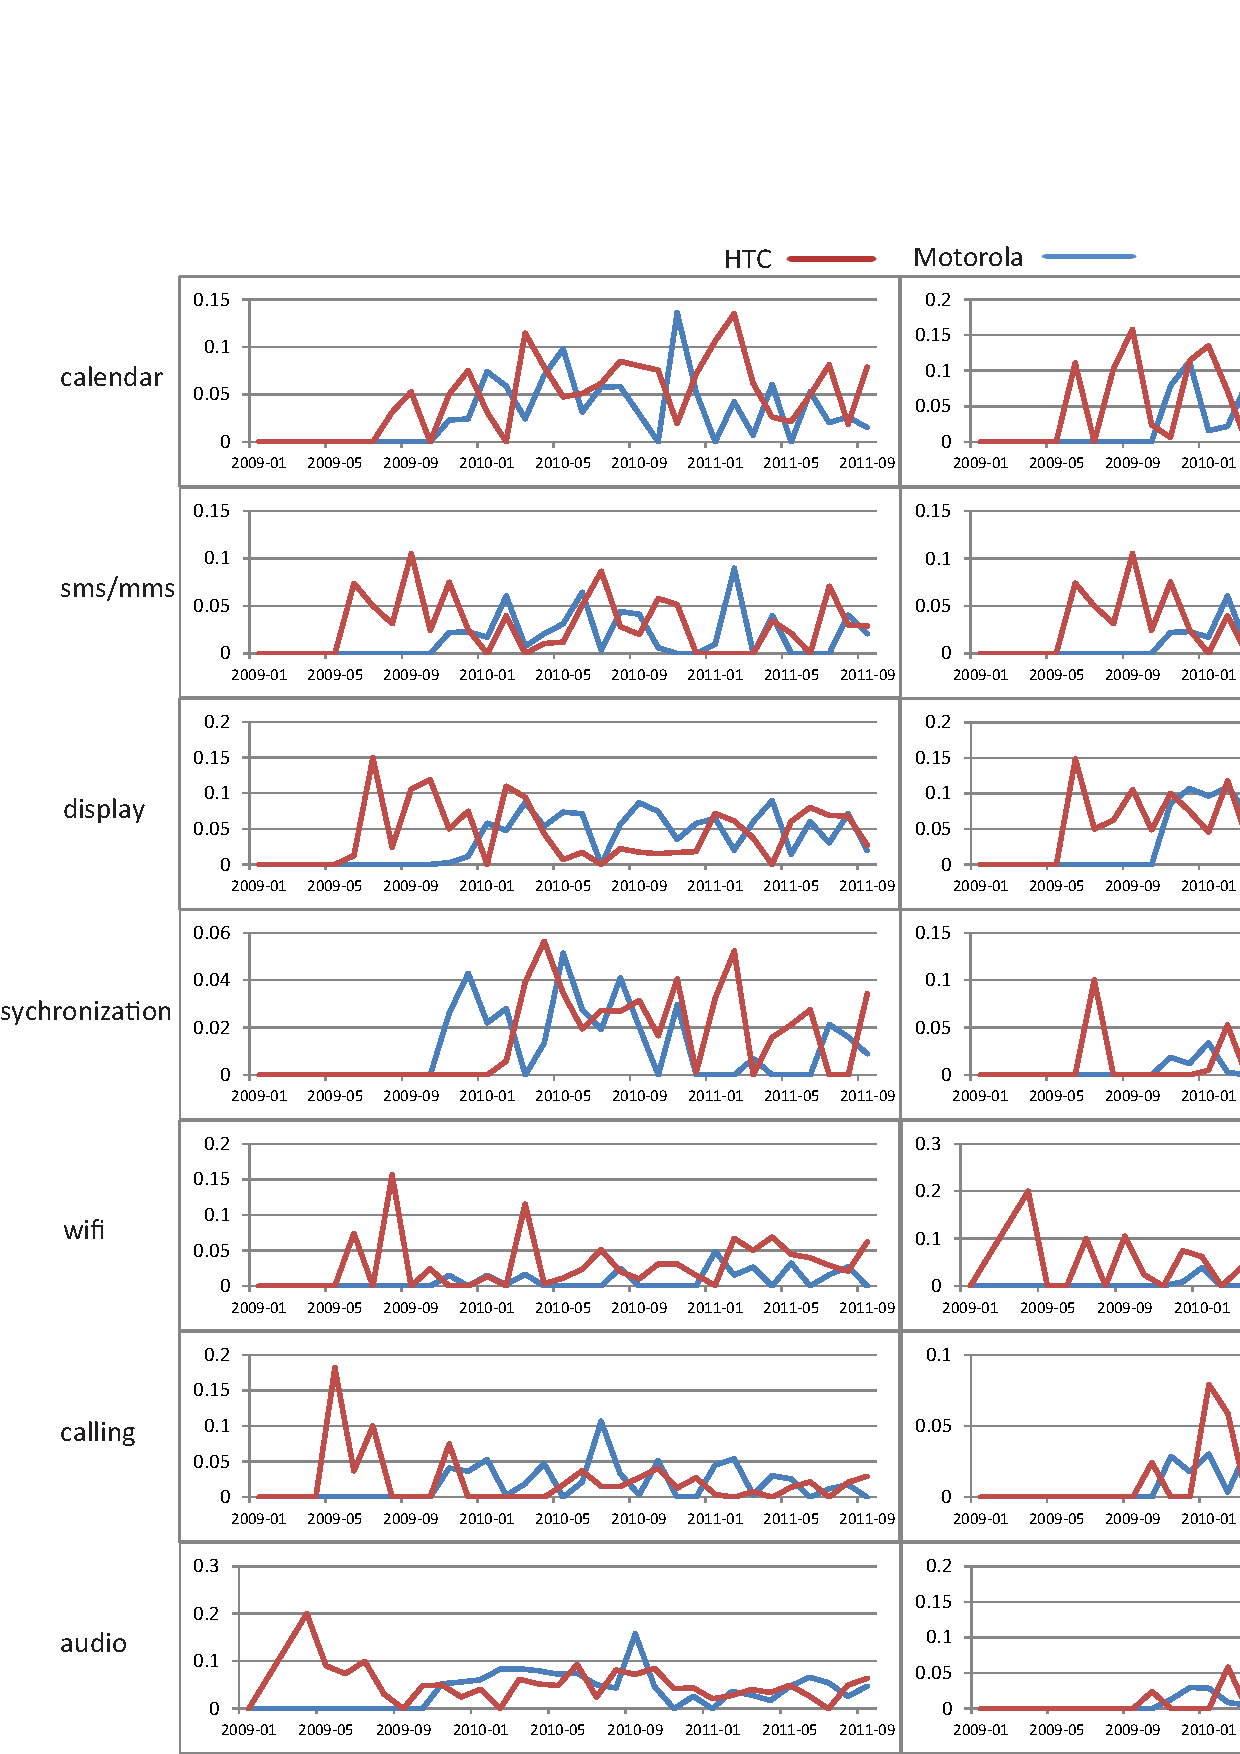
\includegraphics[width=1\textwidth]{commontopic.png}
\caption{Common Troubled Topics in HTC and Motorola}
\label{commontopic}
\end{figure*}

\subsubsection{Common Troubled Topic} 
%space after Table, Figure
%relevance shoule be written as the distribution of the average relevance
Eight \textit{Common Troubled Topics} shared by two vendors are shown in Table \ref{topicslist} and the distribution of average relevance of each topic is shown in Figure \ref{commontopic}. 
%all the labels should be consistent with all the labels in table I.
\textit{Common Troubled Topics} shown in Table \ref{topicslist} for HTC and Motorola share many identical terms. That means they have the same bug reports about sms\/mms(\textit{text, thread, send}), calendar(\textit{event, day, google,appointment,time}), email(\textit{gmail, send, thread}), contact (\textit{number, google,list}), display (\textit{screen,button,behavior}), bluetooth (\textit{headset,connect, calling}), synchronize (\textit{contact, exchange, google}) and setting(\textit{turn,network,mode}). 

We also found that multiple topics share some same terms for each vendor. For HTC, we can see, five topics including sms\/mms, contact, display, bluetooth and setting share the same term ``desire". This indicates that these topics happened frequently in HTC Desire device. Calendar and bluetooth share the same term ``2.2" and ``2.2" means Android version 2.2. This indicates that these two topics happened frequently for Android 2.2 in HTC devices. For Motorola, seven topics except setting share the same term ``droid" and it means Motorola Droid device. In addition, calendar and synchronize in Motorola share ``milestone" which indicates these two topics discussed mostly in Motorola Milestone device. ``Xoom" shared by display and setting indicate that Motorola Xoom has more bug reports related with these two topics. Furthermore, synchronize associates with both ``Xoom" and ``milestone" terms. This indicates bug reports related with synchronize happened frequently in both Motorola Xoom and Motorola Milestone. 

In Figure \ref{commontopic}, HTC and Motorola share the same trends of the distribution of average relevance of topics. Both of them have continuous spikes and drops for each topic over time. That indicates bug reports associated with these topics have no obvious decreasing trends with Android evolution.
%more explain why android version should make the trend of topics decrease in the ideal case.
In summary, calendar in HTC and display in Motorola are strongly correlated with different Android versions. Bluetooth in both of HTC and Motorola have strong correlation with Android 2.1 and Android 2.2. With Android evolution, these distribution of average relevance of each topic for both vendors do not demonstrate the decreasing trend with Android evolution as we expect. Both of vendors have some topics associated with their typical devices. For HTC, five out of eight topics have correlation with HTC Desire device. For Motorola, seven out of eight topics have correlation with Motorola Droid device. As the topics corresponds to the features in Android, we can see these eight features demonstrate the compatibility issues.

\begin{figure*}[htb]
\centering
\includegraphics[width=1\textwidth]{fixtopic.png}
\caption{Common Improved Topics in HTC and Motorola}
\label{fixtopic}
\end{figure*}

\subsubsection{Common Improved Topic}

Six \textit{Common Improved Topics} shared by two vendors are shown in Table \ref{topicslist} and the distribution of the average relevance of each topic is shown in Figure \ref{fixtopic}.

\textit{Common Improved Topics} shown in Table \ref{topicslist} for HTC and Motorola share many identical terms for wifi (\textit{connection,ssid,network}), upgrade (\textit{2.2,2.1,http}), and image(\textit{gallery,picture,photo}). Bug reports associated with upgrade were result from upgrading from Android 2.1 to Android 2.2 in both vendors. This indicates Android 2.2 might have compatibility issue. 

Meanwhile, the \textit{Common Improved Topics} also own some special terms. For HTC, bug reports related with Calling happened frequently in Android 2.1, and bug reports related with Image and Audio happened frequently in Android 2.2. For Motorola, bug reports related to calling happened frequently in Android 2.2. In addition, four out of six topics have correlation with HTC Desire device. For Motorola, seven out of eight topics have correlation with Motorola Droid device and the other one have correlation with Motorola MileStone device. Therefore, we can see these six topics have strong correlation with the Android hardware devices for each vendor.

From Figure \ref{fixtopic}, we can see both HTC and Motorola have spikes in the early stage, and then stay in their values. It indicates the corresponding features of Android tend to be more robust over time with Android evolution during the whole observed period.

In summary, we can see that Calling from both vendors have different correlation with Android versions. With the evolution of Android system, these distributions of average relevance of topics do demonstrate the improved trends with Android evolution as we expect. These topics still have strong correlation with their typical devices for both vendors. Therefore, we can see these six topics demonstrate that the features which have the positive correlation with Android evolution still have strong correlation with their typical devices for both vendors.
% The above summary is not clear to me.

%\begin{figure*}[htb]
%\centering
%\includegraphics[width=1\textwidth]{uniquehtc.png}
%\caption{Unique Topics relevance in HTC}
%\label{uniquehtc}
%\end{figure*}

%\begin{figure*}[htb]
%\centering
%\includegraphics[width=1\textwidth]{uniquemoto.png}
%\caption{Unique Topics relevance in Motorola}
%\label{uniquemoto}
%\end{figure*}


\begin{figure*}[htb]
\centering
\includegraphics[width=1\textwidth]{uniquehtc.png}
\caption{Unique Topics relevance in HTC}
\label{uniquehtc}
\end{figure*}

\begin{figure*}[htb]
\centering
\includegraphics[width=1\textwidth]{uniquemoto.png}
\caption{Unique Topics relevance in Motorola}
\label{uniquemoto}
\end{figure*}


\subsubsection{Unique Topics}

There are the two unique topics for HTC shown in Table \ref{topicslist}. Figure \ref{uniquehtc} shows the distribution of the average relevance of each topic.

\textit{HTC Unique Topics} in Table \ref{topicslist} indicates that HTC has the topic of language (\textit{arabic, desire, language, 2.2, letters, characters, translation, character, read}) topic. The associated terms indicate that bug reports related with language happened frequently in Android 2.2. This stems from the fact that the keyboard multiple language function is a new function introduced in Android 2.2. Moreover, most of HTC devices have no physical keyboard, so this new function has been used frequently by HTC users. In contrast, for Motorola, most of devices have the physical keyboard, so this function has seldom been used. This fact can also be the reason why HTC has ``on-screen" and ``virtual" terms for Keyboard, while Motorola does not have these terms at all.

In Figure \ref{uniquehtc}, HTC keyboard turns to stay steady, while Motorola has spikes and drops over time. HTC language has the relevance distribution, while there are few bug reports related with language to make language as a topic in Motorola.

There are two unique topics for Motorola shown in Table \ref{topicslist}. Figure \ref{uniquemoto} shows the distribution of the average relevance of each topic.

\textit{Motorola Unique Topics} in Table \ref{topicslist} represents HTC and Motorola share the identical terms for GPS (\textit{gps, data, position, location, maps, google, time, lock, wrong, icon, turn, home, latitude}) and browser (\textit{Browser, page, text, http, open, server}). Furthmore, they have special terms separately. For browser, Motorola has “droid”, “milestone” and “xoom” terms together. This indicates that the browser bug reports happened frequently in three Motorola devices. This indicates that browser has portability issue within Motorola Android devices.

In Figure \ref{uniquemoto}, comparing two vendors, we can see the distribution of the average relevance for GPS and browser demonstrate different trends. For HTC, they have strikes and drops in the early stage, and then stay steady. For Motorola, they stay steady and then have strikes and drops afterwards.
% I am not clear about your summary here.
In summary, for different vendors, these unique topics show significantly different relevance as a result of the different devices. Within the same vendor, the associated terms implicate that some features have portability issues across devices.For example, browser in Motorola.

\section{Discussion of Fragmentation}
%What is feature evolution?
According to the analysis about \textit{Common Troubled Topics}, we can see that there is no strong correlation between the feature evolution and Android evolution. In addition, The topic - upgrade has strong correlation with Android 2.1 and Android 2.2. As there are some features evolution demonstrate stable trends with Android evolution implicated by the \textit{Common Improved Topics}, we can conclude that Android has compatibility issue in some features.

From \textit{Common Improved Topics} and \textit{Unique Topics}, we can see the same topic from different vendors have different correlation, and they have strong correlation with some specific vendors' devices. These observations reveal that Android has portability issue in some features.

When we refer to Android, we generally mean all Android versions existing in the world which include both Android branches from Android community and that from vendors. In the sense of Android itself, we can see that Android has software fragmentation issue. We also discover that there are some features has strong correlation with vendors' devices. In the sense of Android devices from different vendor, we can conclude that Android has hardware fragmentation as well.


%\begin{figure}[!htb]
%\centering
%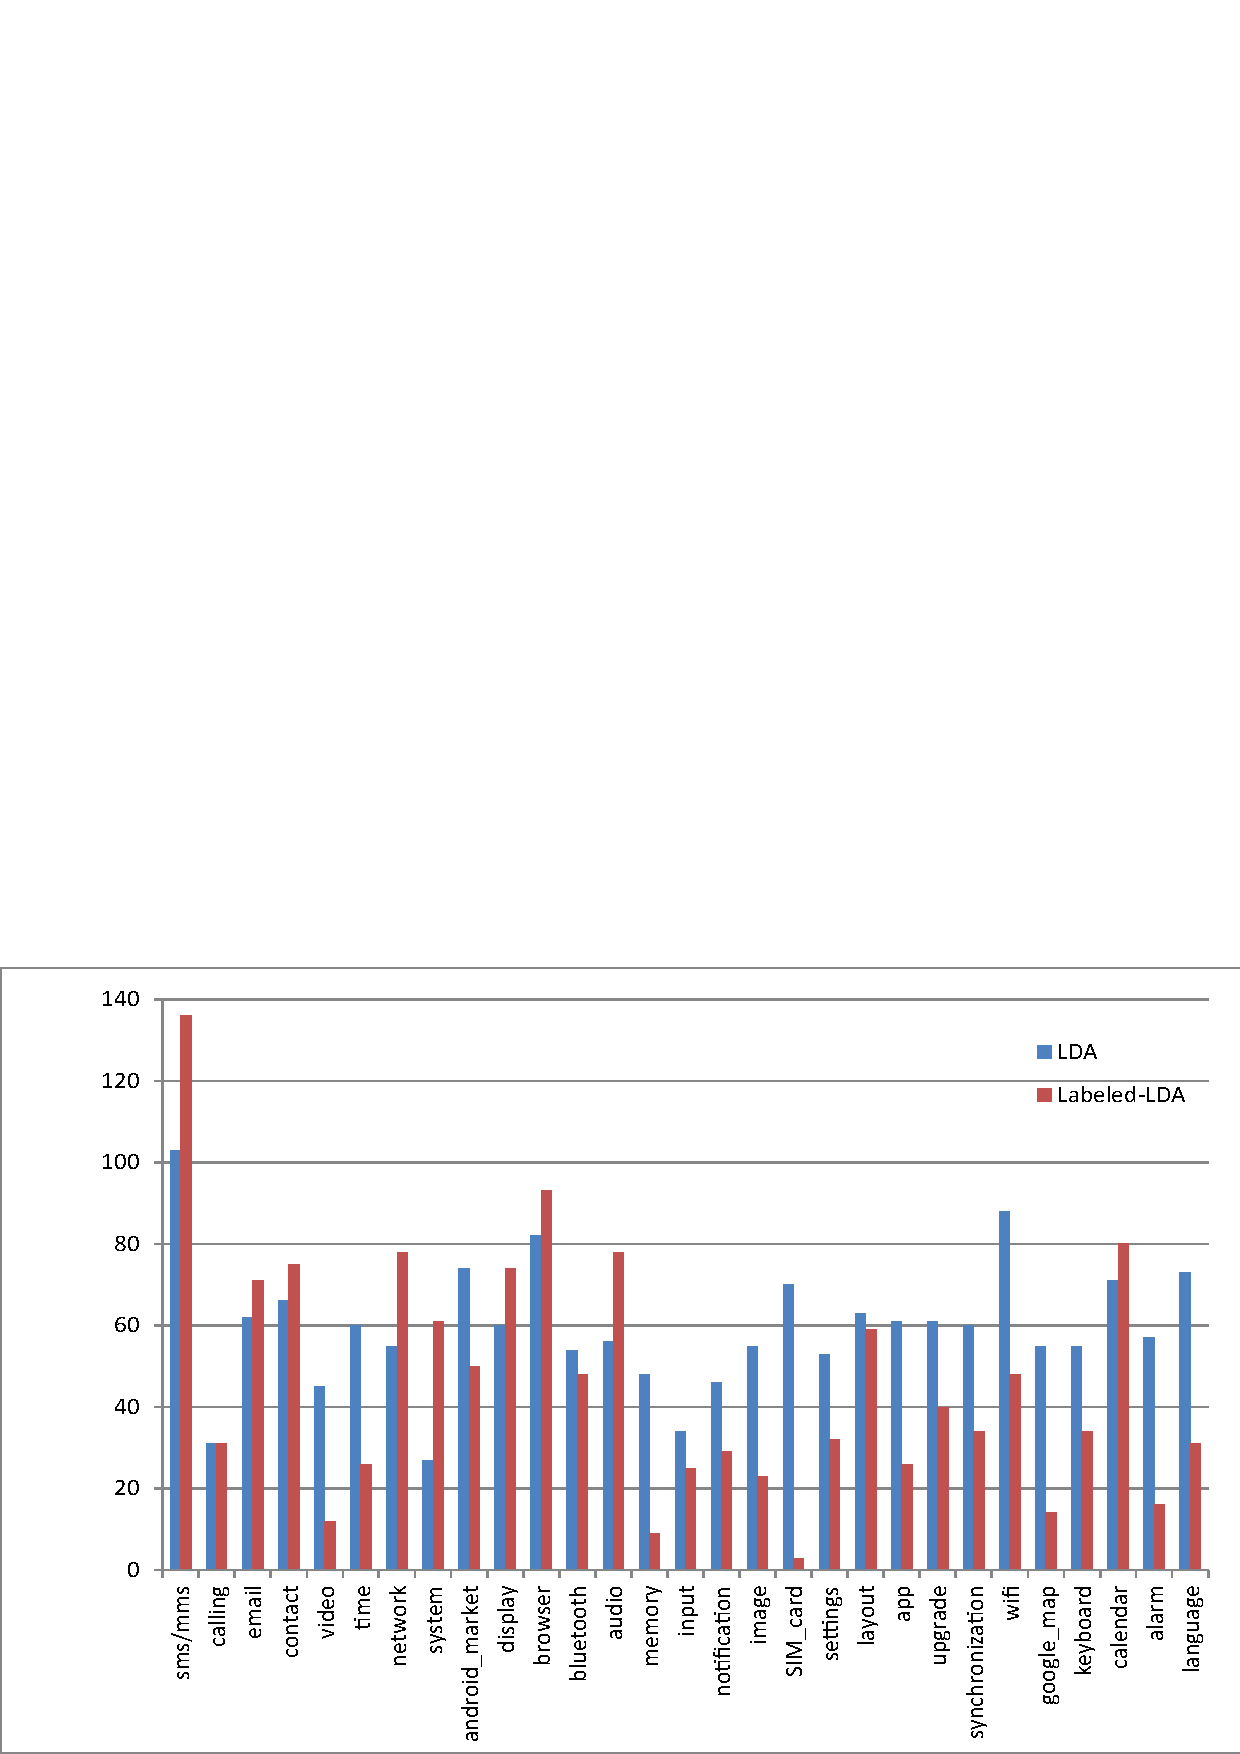
\includegraphics[width=0.4\textwidth]{htcldallda.png}
%\caption{Comparison of number of bug reports related to the same labels from LDA and labeled-LDA in HTC. The X axis is the same labels from LDA and labeled-LDA and the Y axis is the number of bug reports.}
%\end{figure}
%
%\begin{figure}[!htb]
%\centering
%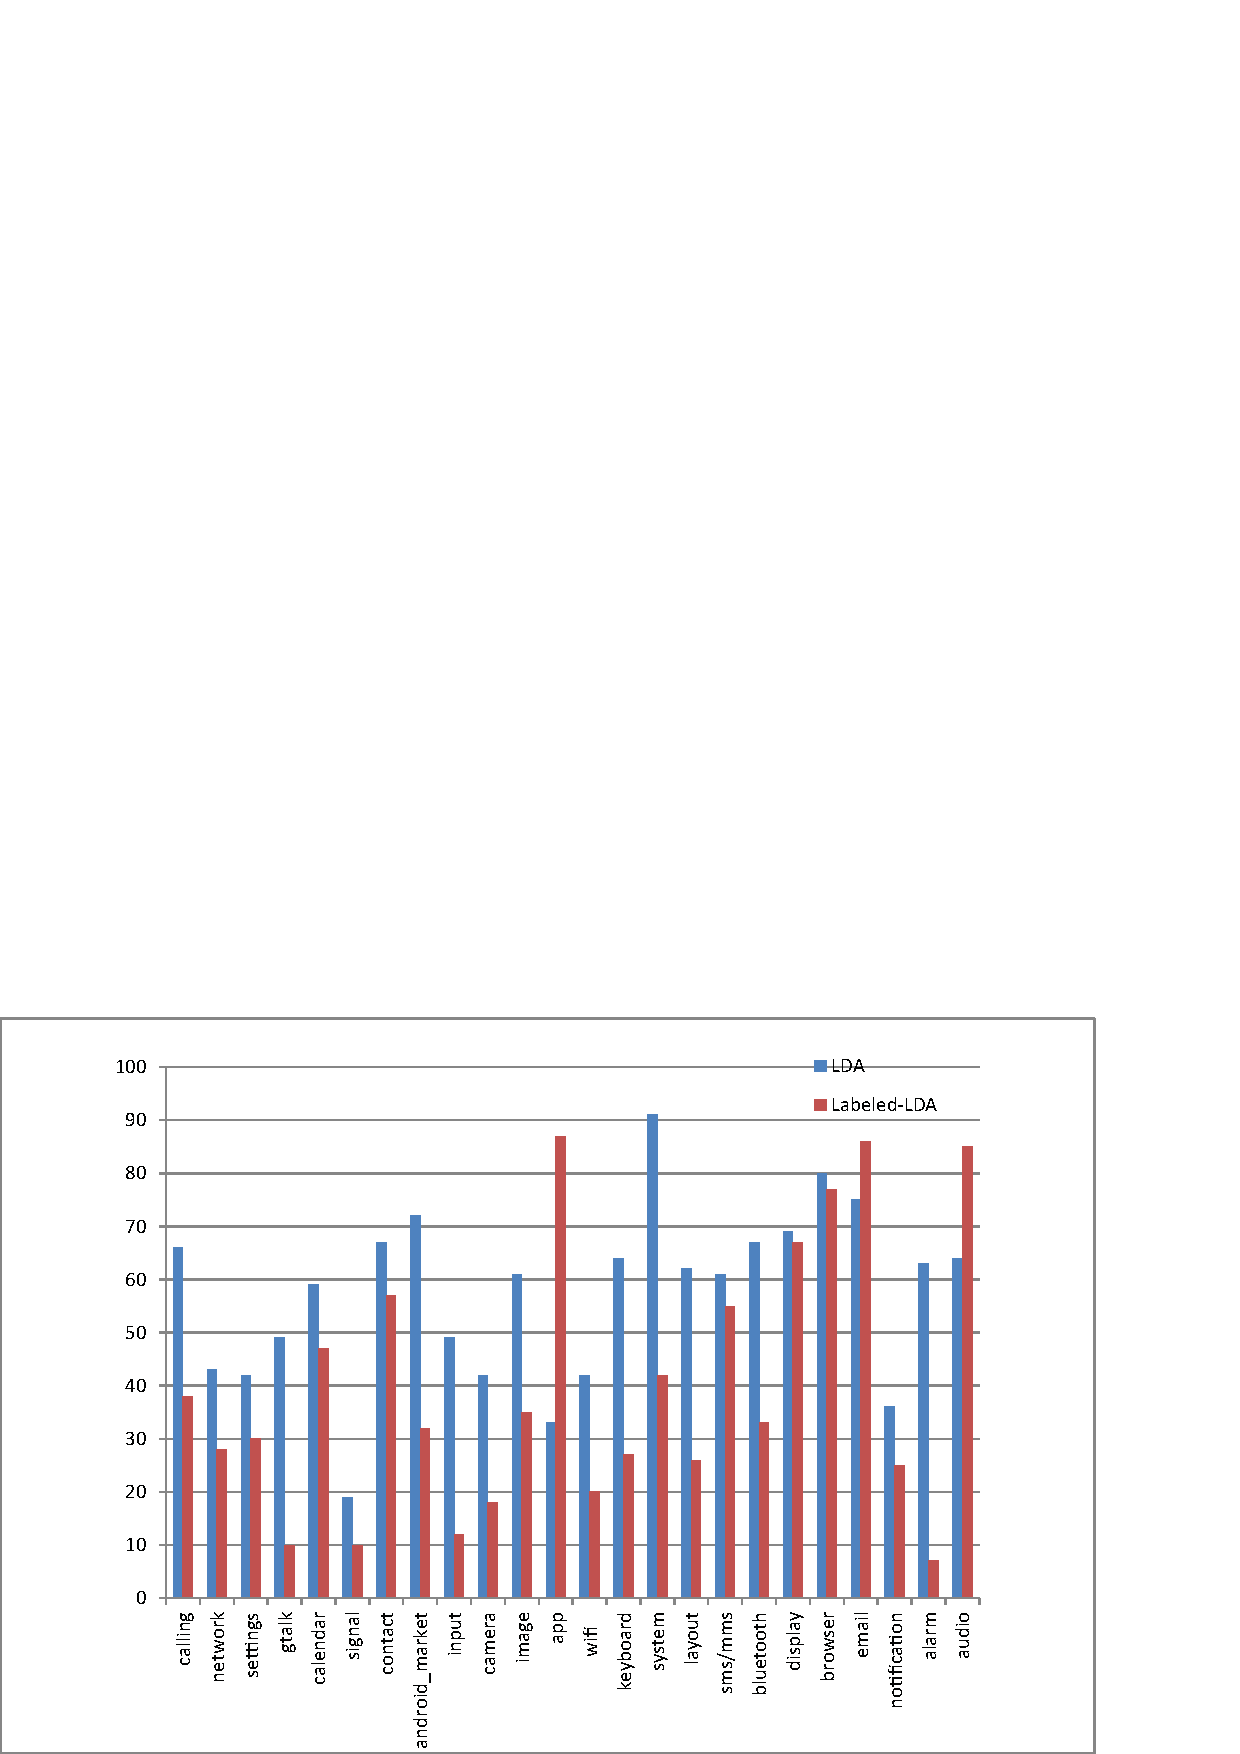
\includegraphics[width=0.4\textwidth]{motoldallda.png}
%\caption{Comparison of number of bug reports related to the same labels from LDA and labeled-LDA in Motorola. The X axis is the same labels from LDA and labeled-LDA and the Y axis is the number of bug reports.}
%\end{figure}
%
%\begin{figure}[htb]
%\centering
%\includegraphics[width=0.4\textwidth]{htcratiosim.png}
%\caption{The comparison of ratio and similarity in HTC. The result of the smaller number of bug reports related to this label in LDA or labeled-LDA divided by the larger one is the ratio of this label. The X axis is the same labels from LDA and labeled-LDA.}
%\end{figure}
%
%\begin{figure}[htb]
%\centering
%\includegraphics[width=0.4\textwidth]{motoratiosim.png}
%\caption{The comparison of ratio and similarity in Motorola. The result of the smaller number of bug reports related to this label in LDA or labeled-LDA divided by the larger one is the ratio of this label. The X axis is the same labels from LDA and Labeled LDA.}
%\end{figure}


%\begin{figure*}[htb]
%\centering
%\includegraphics[width=1\textwidth]{bugovertime.png}
%\caption{Number of bugs with the major version of Android for HTC and Motorola}
%\label{bugovertime}
%\end{figure*}




%\begin{figure*}[htb]
%\centering
%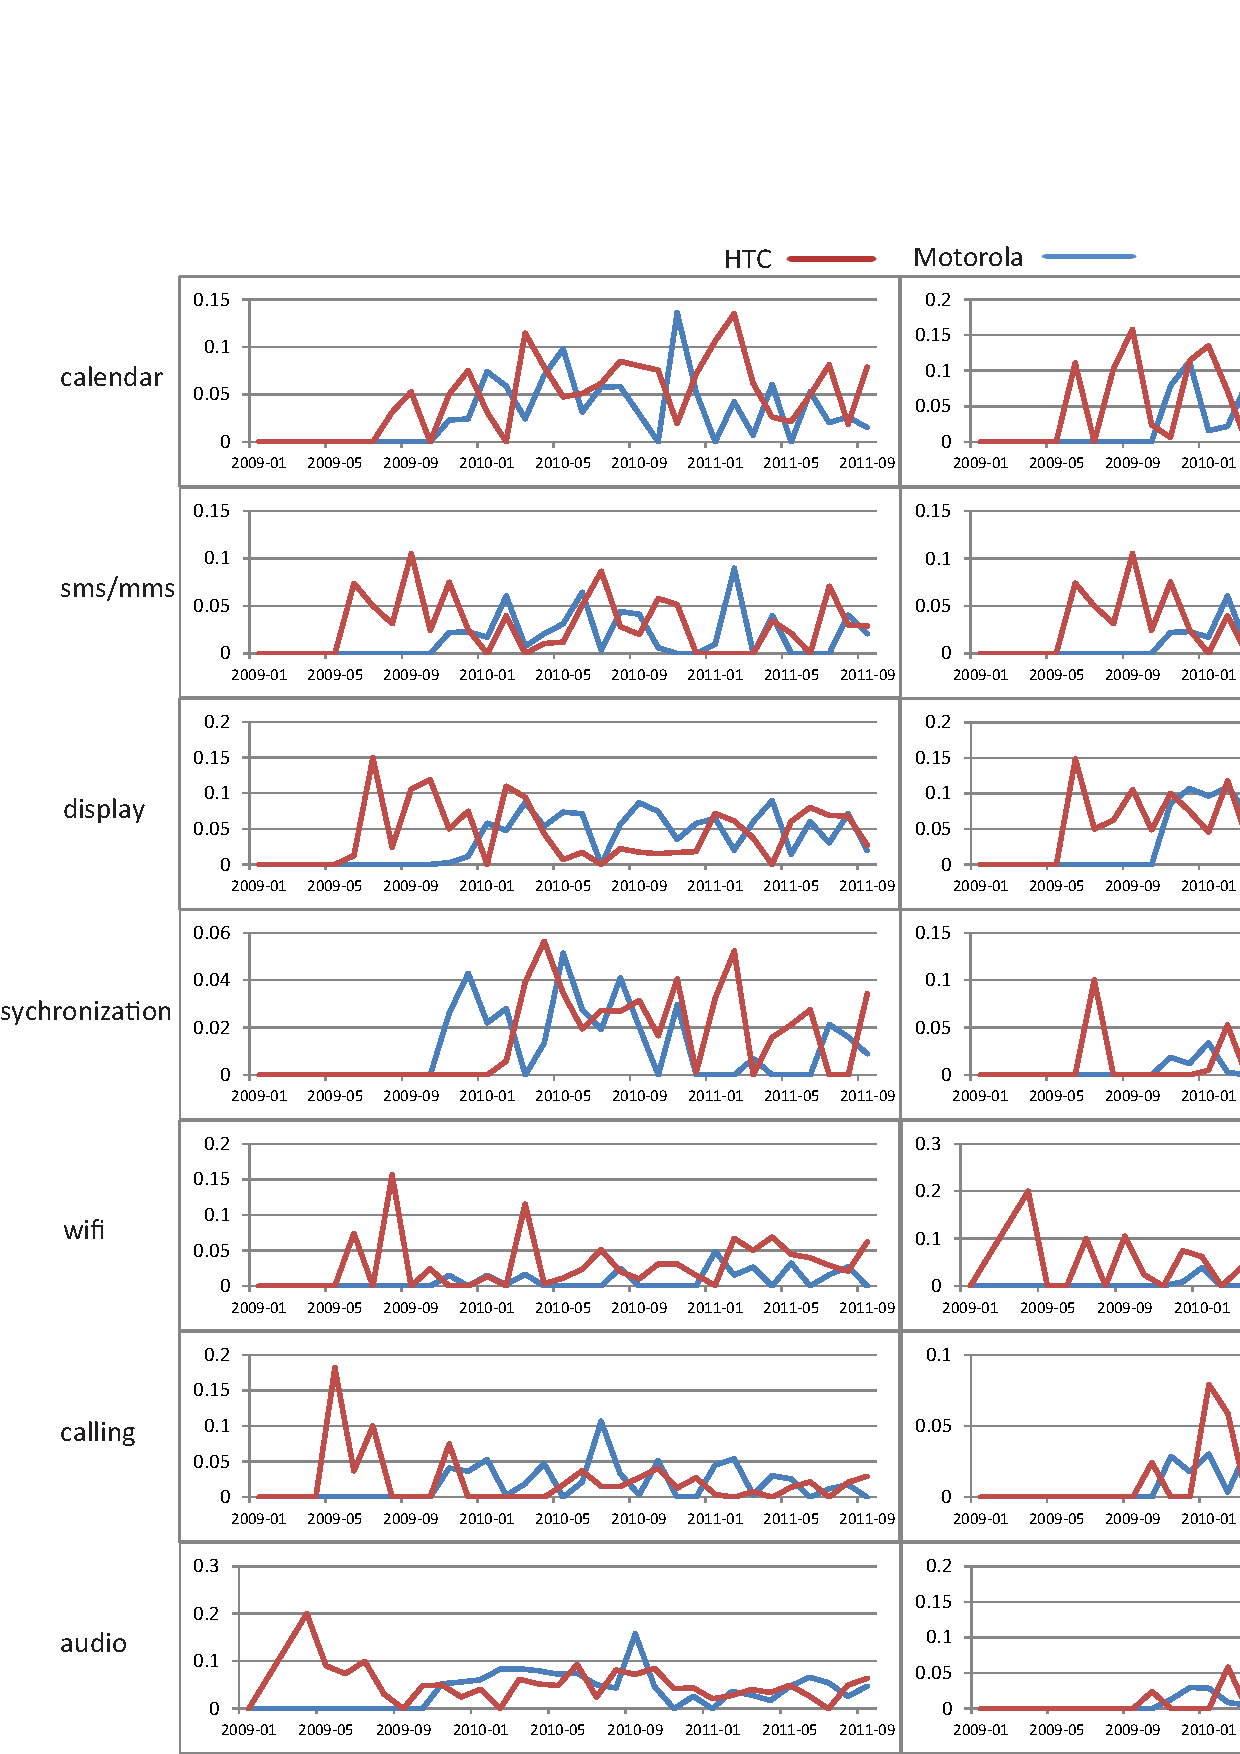
\includegraphics[width=1\textwidth]{commontopic.png}
%\caption{Common Troubled Topics in HTC and Motorola}
%\label{commontopic}
%\end{figure*}


%\begin{figure*}[htb]
%\centering
%\includegraphics[width=1\textwidth]{fixtopic.png}
%\caption{Common Improved Topics in HTC and Motorola}
%\label{fixtopic}
%\end{figure*}

\section{Comparing of LDA and Labeled-LDA}
In this section we investigate if LDA and Labeled-LDA would generate the similar results.

Figure \ref{similarityhtc} and Figure \ref{similaritymoto} depict the pairwise Jaccard similarities of labels from LDA and Labeled-LDA. The brighter spots mean the pair of labels have higher Jaccard similarity. These two labels in LDA and Labeled-LDA would be relevant to more similar set of bug reports. The darker spots mean the pair of labels have lower Jaccard similarity and share less bug reports in common. 

From these two Jaccard similarity plots (Figure \ref{similarityhtc} and Figure \ref{similaritymoto}) of labels between LDA and Labeled-LDA, we can observe that most of the Jaccard similarity values are quite small except a few diagonal ones, especially in HTC. This observation is expected since most of the diagonal spots are the Jaccard similarities between the same labels from LDA and Labeled-LDA. However, even the mean similarities of the diagonal spots are just about 0.2 for HTC and 0.08 for Motorola. The similarity plot for Motorola has much more noises than the plot for HTC.  

Figure \ref{bughtc} shows the number of bug reports that related to the same labels in the bug reports of HTC and Figure \ref{bugmoto} illustrates the number of bug reports that related to the same labels in the bug reports of Motorola. The $ p $ values of the Chi-squared test on the two sets of distribution are both close to zero. Hence the number of bug reports related to same labels in LDA and Labeled-LDA are quite different.

\begin{figure*}[htb]
\centering
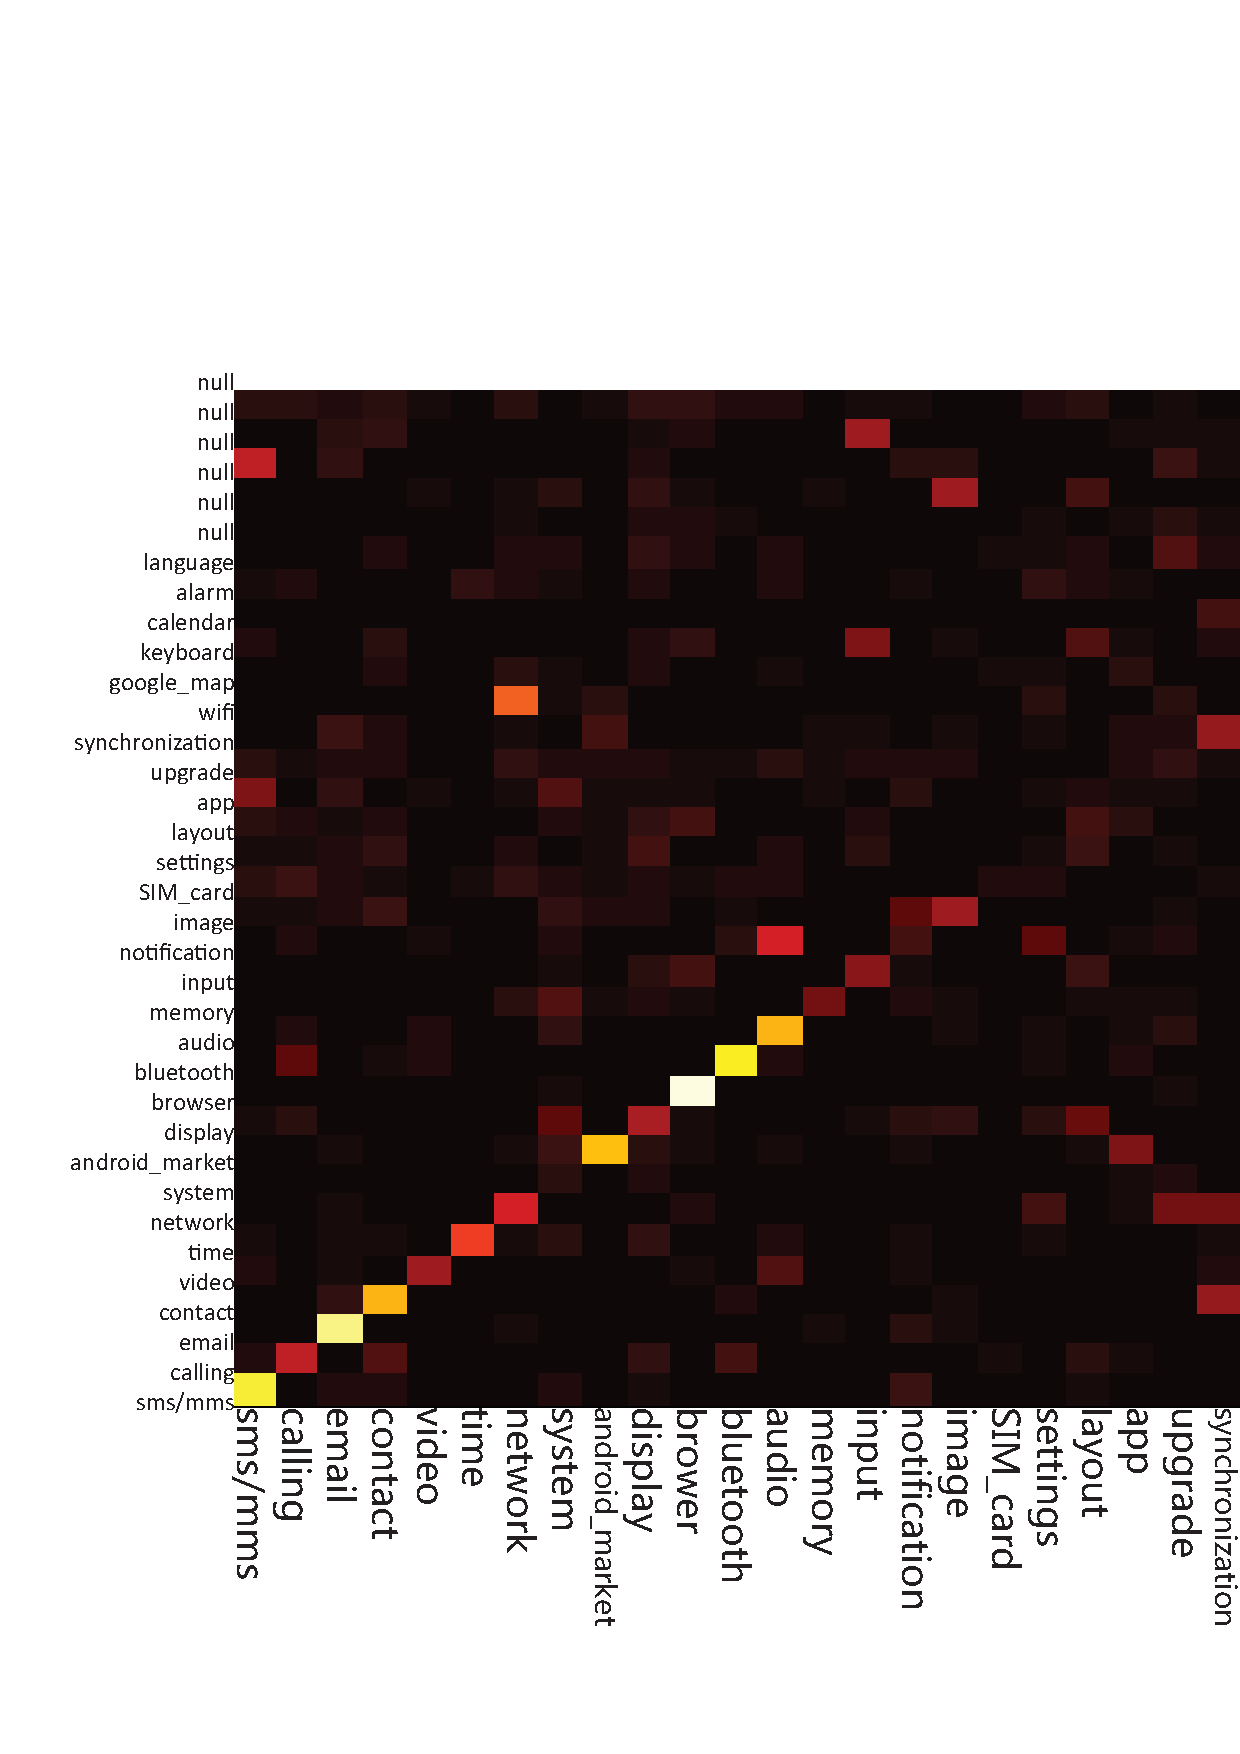
\includegraphics[width=1\textwidth]{htcsim.png}
\caption{Jaccard similarity of labels between LDA and Labeled-LDA in HTC. X axis is the labels in labeled-LDA and Y axis is the labels of topics generated by LDA. The label ``null" in the Y axis means that topic cannot be labeled. The result is based on the HTC bug reports under the threshold of document relevance of 0.2. Brighter means higher Jaccard similarity.}
\label{similarityhtc}
\end{figure*}

\begin{figure*}[htb]
\centering
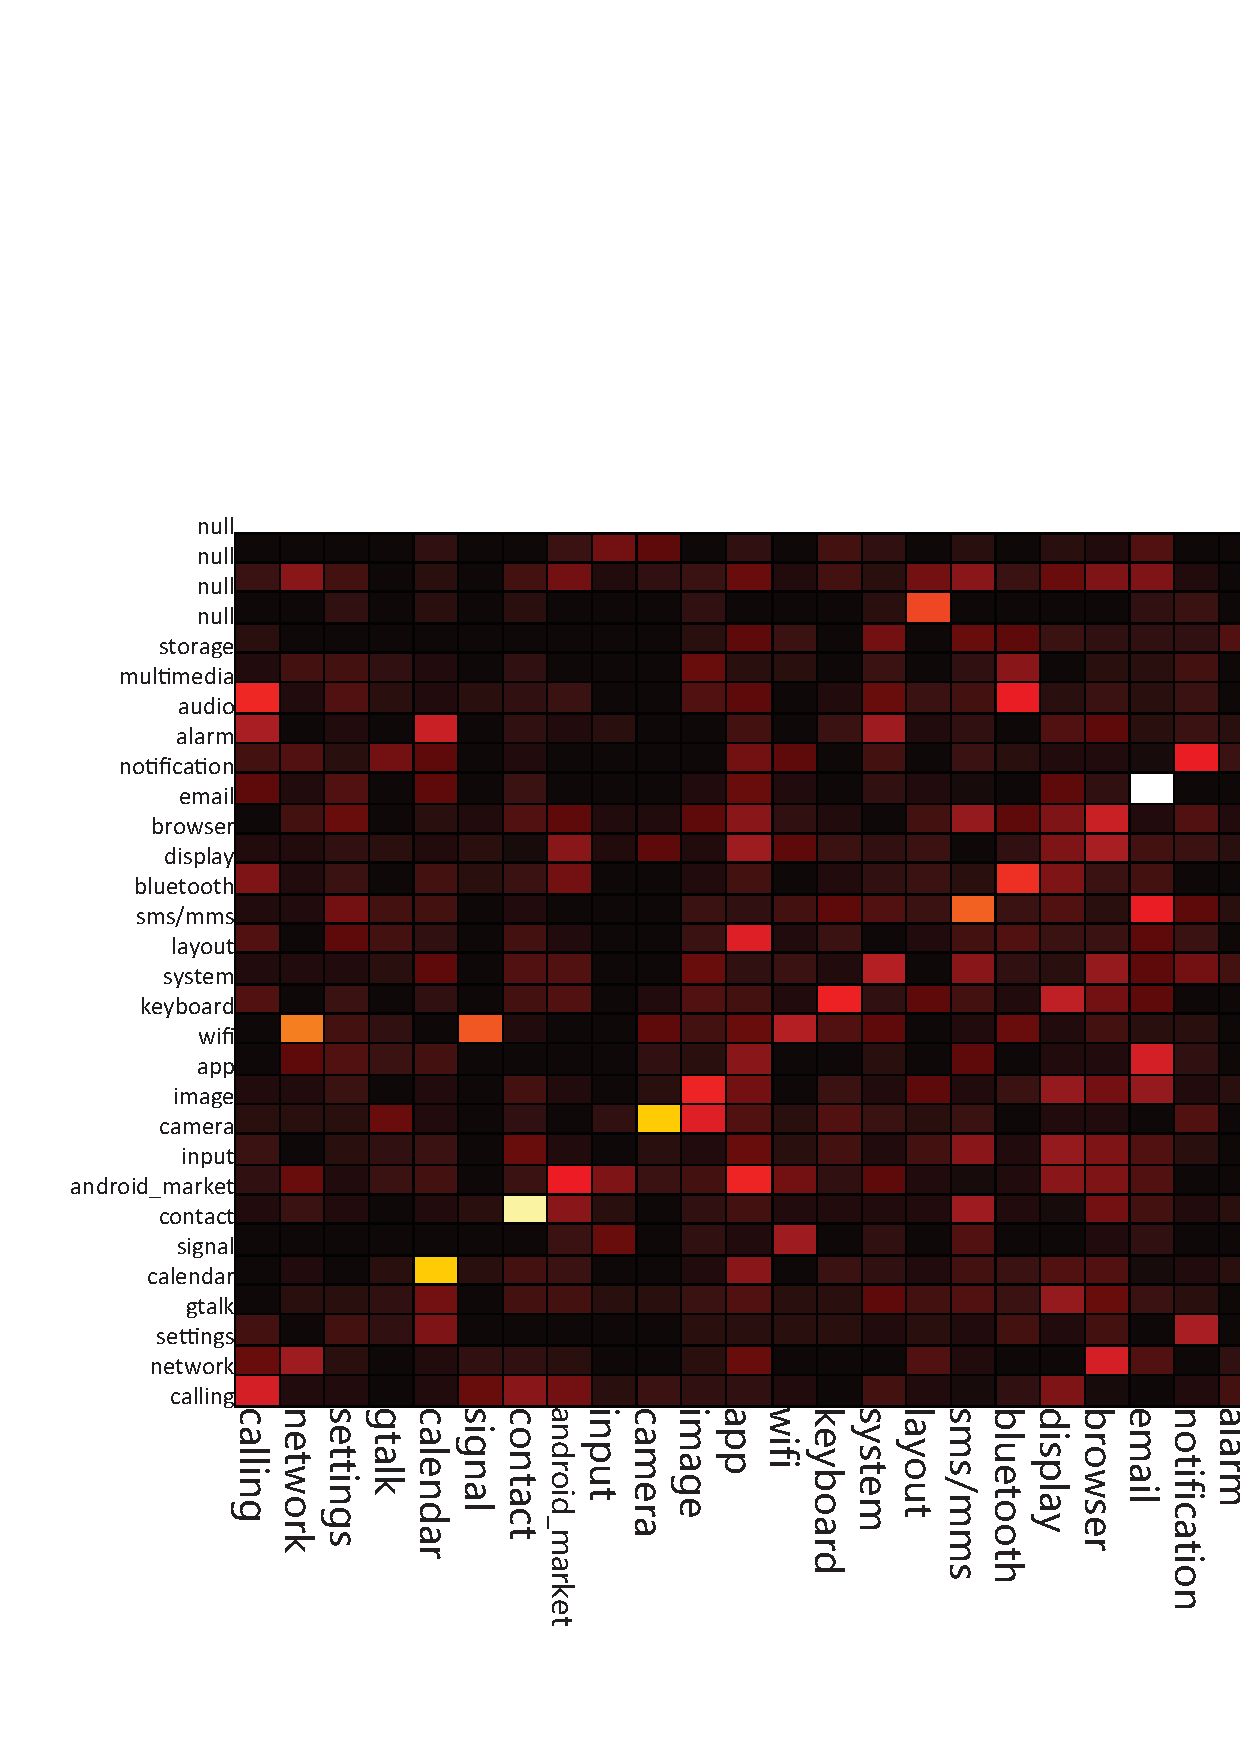
\includegraphics[width=1\textwidth]{motosim.png}
\caption{Jaccard similarity of labels between LDA and Labeled-LDA in Motorola. X axis is the labels in labeled-LDA and Y axis is the labels of topics generated by LDA. The label ``null" in the Y axis means that topic cannot be labeled. The result is based on the Motorola bug reports under the threshold of document relevance of 0.2. Brighter means higher Jaccard similarity.}
\label{similaritymoto}
\end{figure*}

\begin{figure}[htb]
\centering
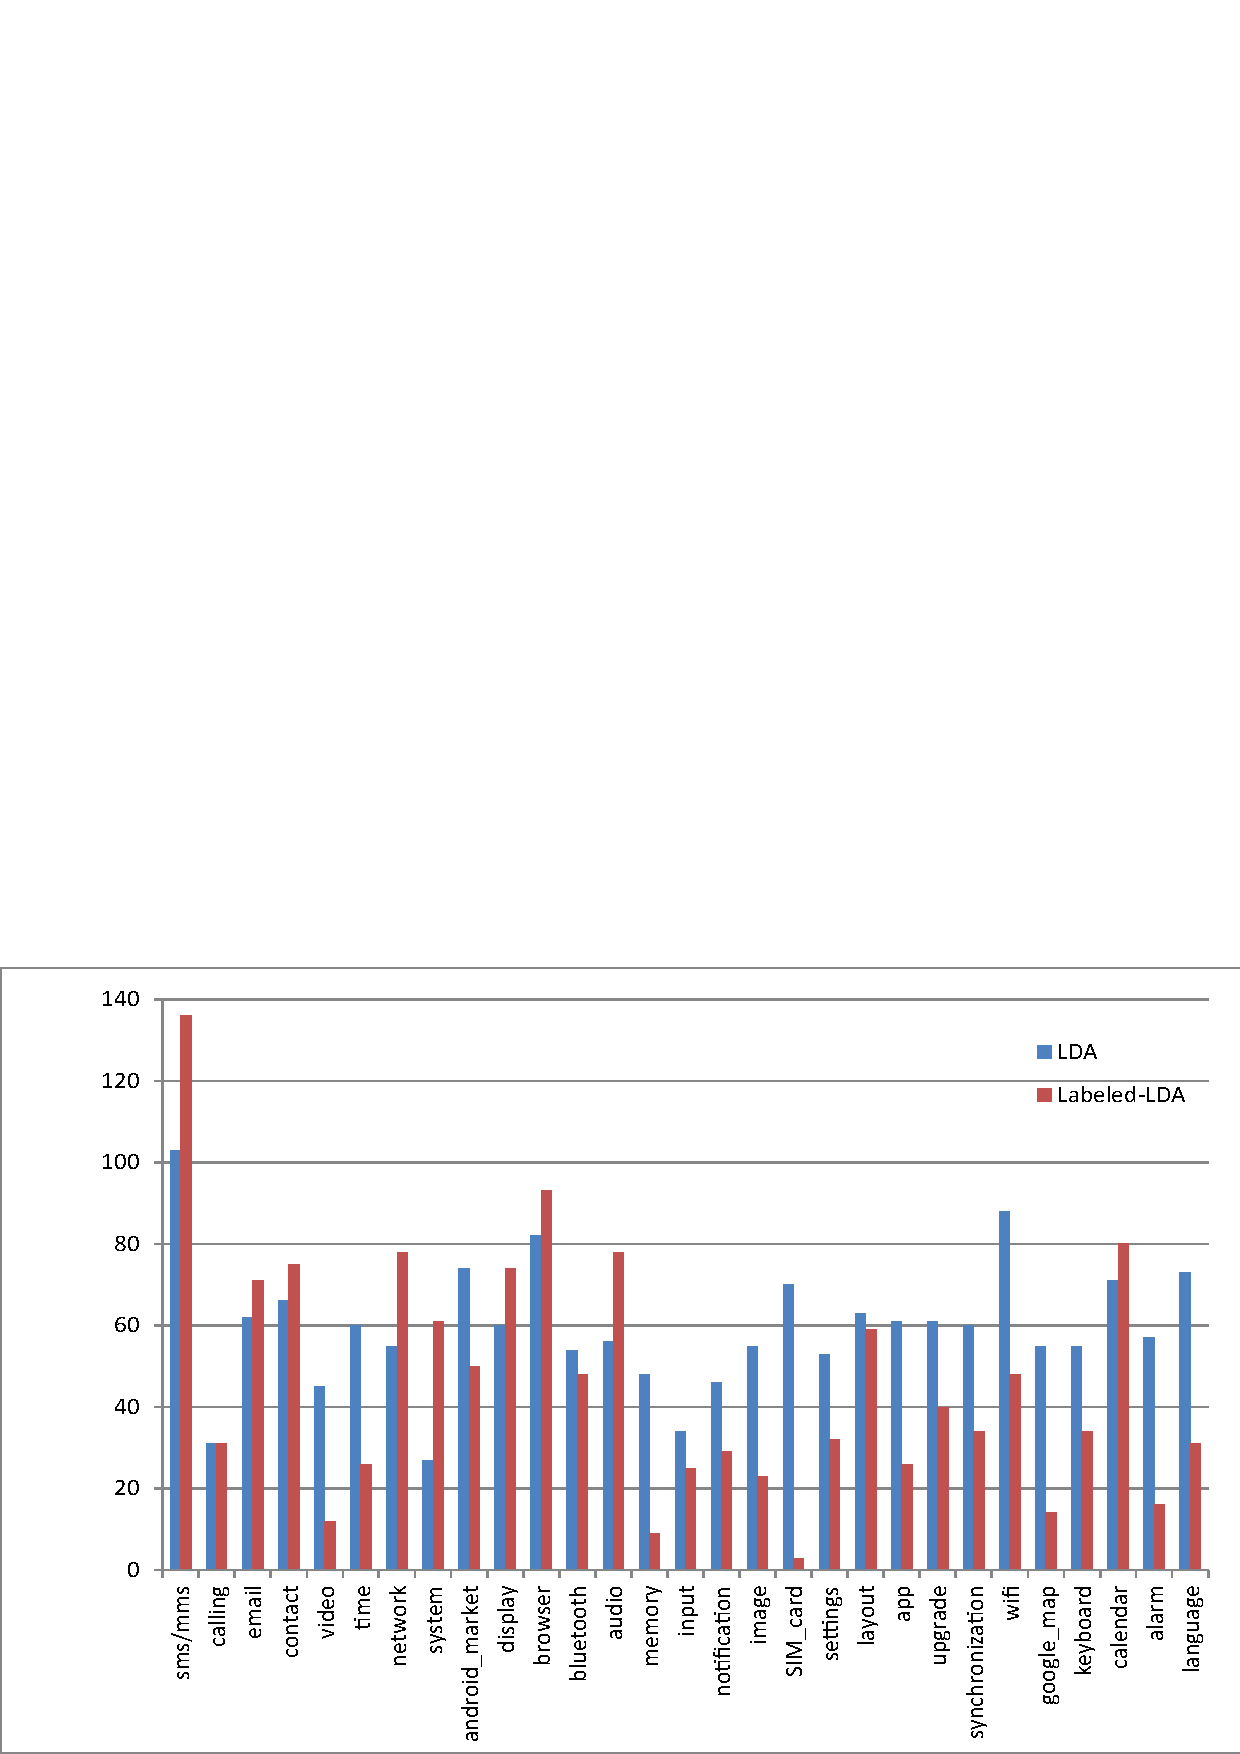
\includegraphics[width=0.5\textwidth]{htcldallda.png}
\caption{Comparison of number of bug reports related to the same labels from LDA and labeled-LDA in HTC. The X axis is the same labels from LDA and labeled-LDA and the Y axis is the number of bug reports.}
\label{bughtc}
\end{figure}

\begin{figure}[!htb]
\centering
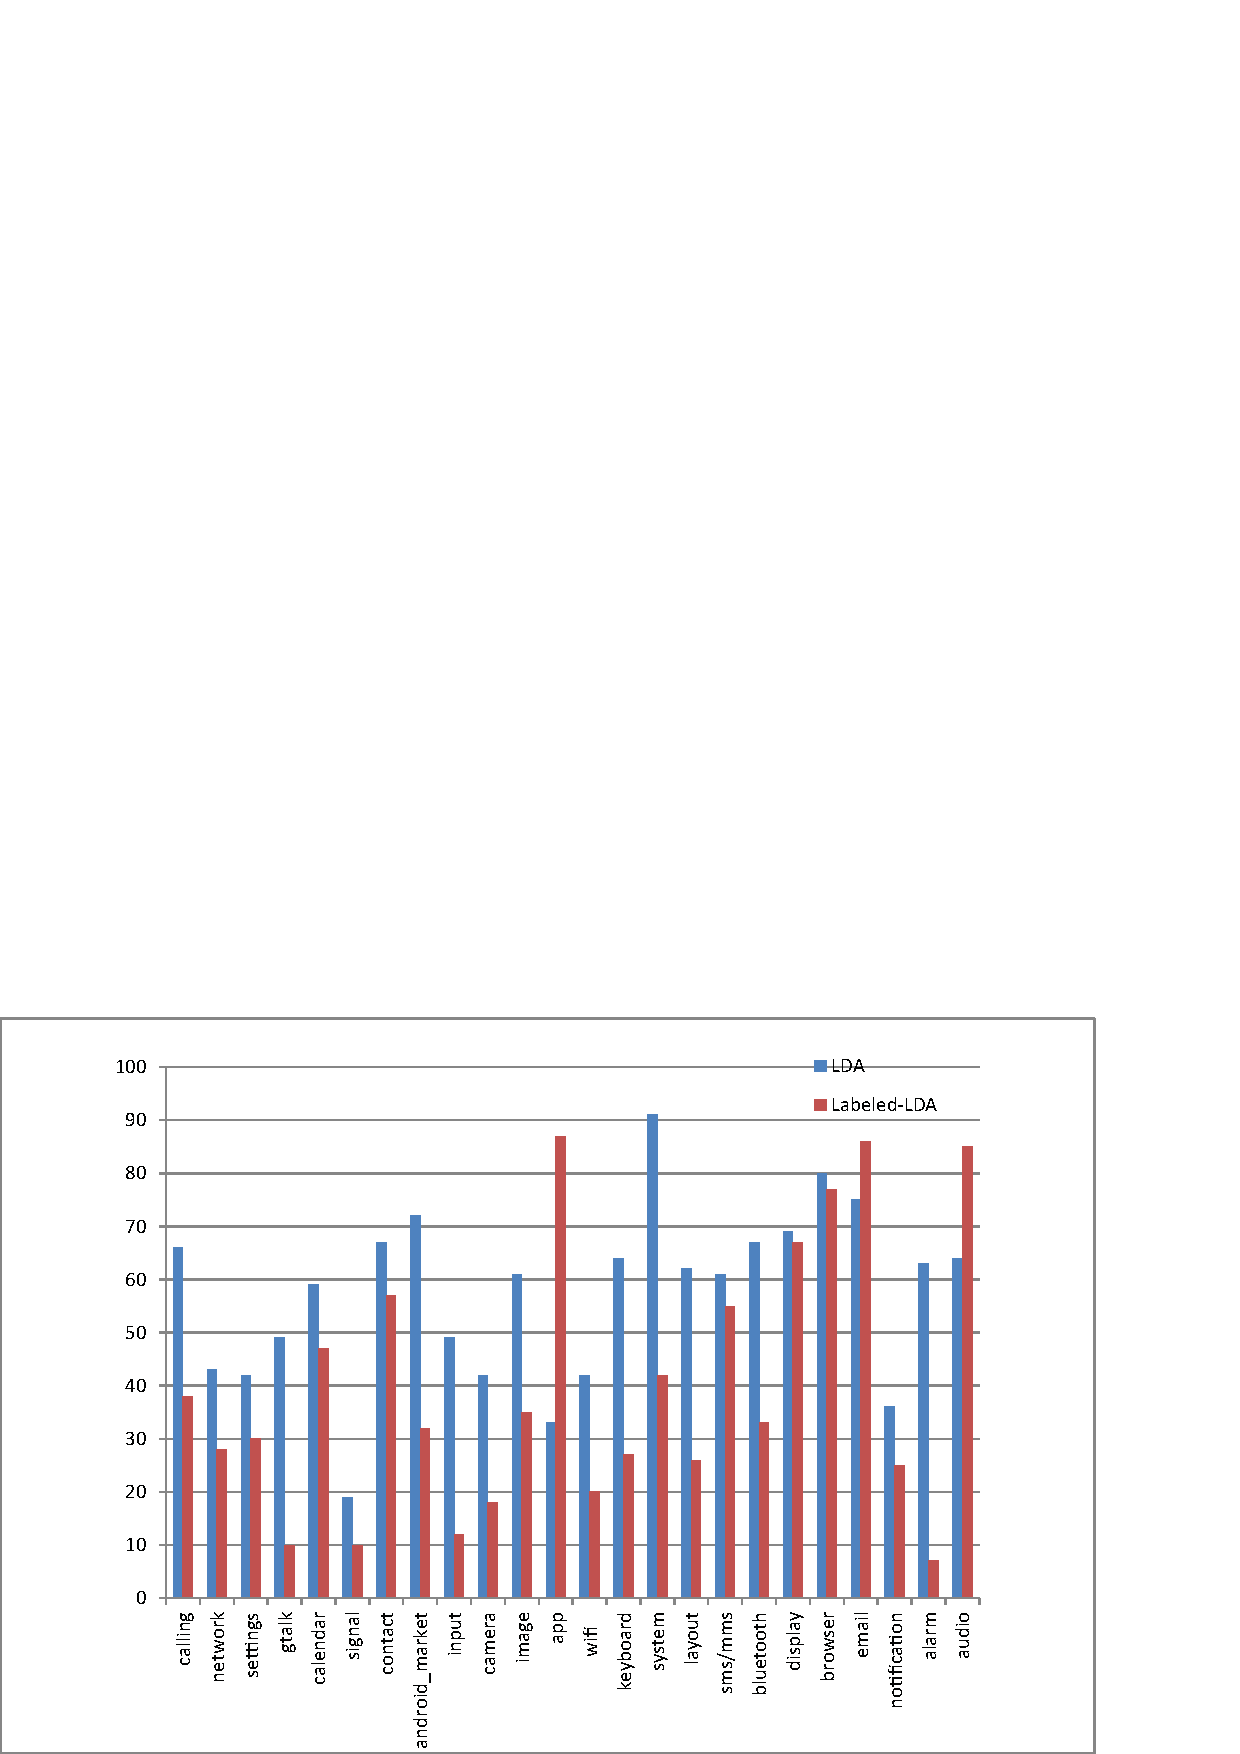
\includegraphics[width=0.5\textwidth]{motoldallda.png}
\caption{Comparison of number of bug reports related to the same labels from LDA and labeled-LDA in Motorola. The X axis is the same labels from LDA and labeled-LDA and the Y axis is the number of bug reports.}
\label{bugmoto}
\end{figure}

%Most of the same labels from LDA and labeled-LDA have the comparable amount of bug reports. For example, the label ``calling'' from the HTC bug reports has exactly the same number of bugs related to for both results of LDA and Labeled LDA. However, the similarity of these related bug reports in terms of this label ``calling'' is very low which means LDA and Labeled LDA related quite different bug reports to this label. When doing this comparison, we cannot ignore the number of bugs that related to each label from both two techniques. That is, for one label, the ratio (the smaller number is divided by the bigger number so the ratio is always less or equal to one) of the number of bug reports related to this label predicted by LDA to that of Labeled LDA would be the upper bound of the similarity value. From Figure \ref{bughtc} and Figure \ref{bugmoto} that the relation between topics and each bug report modeled by LDA is quite different from the results generated by Labeled LDA.

%The similarity values for these labels in Figure \ref{similaritymoto} are quite low compared with the ratio. Only about ten labels in HTC have similarity values that are larger than half of the ratio. For Motorola, the similarity values are all very low compared with the upper bound of the similarity values.

We can conclude that only few of the bug reports in HTC and Motorola are predicted by LDA and labeled-LDA to be related to the same labels. In other words, the relation between topics and each bug report modeled by LDA is quite different from the results generated by Labeled-LDA. We think the manual efforts of labeling all the bug reports would help us gain the better topic models generated by Labeled-LDA. 

%\begin{figure}[htb]
%\centering
%\includegraphics[width=0.5\textwidth]{htcratiosim.png}
%\caption{The comparison of ratio and similarity in HTC. The result of the smaller number of bug reports related to this label in LDA or Labeled LDA divided by the larger one is the ratio of this label. The X axis is the same labels from LDA and labeled-LDA.}
%\end{figure}

%\begin{figure}[htb]
%\centering
%\includegraphics[width=0.5\textwidth]{motoratiosim.png}
%\caption{The comparison of ratio and similarity in Motorola. The result of the smaller number of bug reports related to this label in LDA or labeled-LDA divided by the larger one is the ratio of this label. The X axis is the same labels from LDA and labeled-LDA.}
%\end{figure}



\begin{table*}[!htb]
\renewcommand{\arraystretch}{1.3}
% if using array.sty, it might be a good idea to tweak the value of
% \extrarowheight as needed to properly center the text within the cells
\caption{Topics and associated Word List with Related Top 15 Terms}
\label{topicslist}
\centering
\begin{tabular}{|c||c||c||c|}
\hline
Topic Type & Label & HTC & Motorola\\ 
\hline
Common Troubled Topics & sms\//mms &message,	sms,	text, thread, time,  & message, text, sms, droid, send,	\\
&& sent, desire, contact, new, number, &	thread, messaging, sent,user, version,\\ 
&&conversation, send, version, app, screen &version, person, threads, number, http\\ \cline{2-4}

  & email & email, mail, gmail, app, message,   &email, droid, account,	gmail, mail, \\
&&inbox, messages,client,emails, account,  &server, message,user,emails, exchange, \\ 
&&send, interface, thread, time, new & file, version, open, device, app\\ \cline{2-4}
            
& calendar&calendar, event, day, events, google,  &calendar,	event, droid, google, appointment, \\
&&view, 2.2,time,month, date, &events, day, field, date, appointments, \\ 
&&version, reminder, appointment,  edit, running &outlook, milestone, data, app, version\\ \cline{2-4}
            
& contact & contact, contacts, number, freed, activity,  &contact, contacts, droid, number, numbers, \\
&&displayed, list, group, google, numbers,   &address, version, google, menu, correct, \\
&&starting,desire, user, version, field & behavior, different,list, option, gmail\\ \cline{2-4}
            
  & display&screen, version, desire,behavior, app, &droid, screen, button, correct, home, \\
&& home, number,code, final, press,  &display, behavior,  landscape, 2.1,  menu, \\
&&sure, user, black, new, power  &bar, xoom,device, user, status\\ \cline{2-4}
   
& bluetooth & bluetooth,headset, car, connect, device,  &bluetooth,	headset, droid, device,connected, \\
 &&connection, version, data, app, desire, & connect, devices, calls,car,issue,	\\
&&desire,	2.2, work, connects, behavior,2.1 & connection, 2.2, car,pair, time\\ \cline{2-4}
            
  & synchronize&contacts, account, sync, exchange, contact, &sync, google, account, contacts, device, \\
&&google, ears, device, group, server, &contact, group, time, exchange, contacts, \\
&&Gmail, policy, new, list, display&display, groups,  list,  droid, milestone\\ \cline{2-4}
            
  & settings&volume, sound,	set, pattern,  default,&settings, device, menu, turn,	network, \\
 && turn, desire, static, control, apps,&vpn, honeycomb, button, xoom,  settings, \\
  && change, settings, media, dns, screen &behavior,	right, wireless, headset, mode\\
\hline

Common Improved Topics 
&wifi & wifi, access, network, connection, connect, &wifi, xoom, connect, hotspot, turn, \\
&&router, ssid, desire, http, wi-fi,&connection, ssid, radio, error,signal, \\

&&device, connected, scan, point, app &state, user, time, feature,hotspots\\ \cline{2-4}

&upgrade & update, 2.2, file, 2.1, google  & update, droid, 2.1,2.2, home, \\

 &&version, error, upgrade, froyo, install, & http, version, user, issue, device,\\           
 
 &&work, desire, ota, card, ssl & longer, settings, performance, issues, updated\\            \cline{2-4}
          
&audio& music, audio, player, file, play, &music, droid, player, media, audio,  \\

&&2.2,sound, version, time, playing, & files, volume, play, playing, version,\\

&&playback, app, start, reproduce, mp3 &app, issue, mode, running, genre, sound, user\\ \cline{2-4}
           
&calling& number, calls, calling, 2.1, receive, &droid, calls, number, end, button, \\
&& called, button, answer, bluetooth, desire,  &answer, incoming, screen, voice, speaker, \\ 

&& screen, incoming, works, time, magic & speaker, 2.2, device, place, headphones\\ \cline{2-4}
           
&android market& market, app, google, account, download, &market, apps, app, device, application,  \\

&&update, application, user, device, version, &update, open, user, version, time, \\ 
           
&&apps, paid, desire, installed, application & reporoduce, download, purchase, google, milestone\\ \cline{2-4}   
        
&image & image, gallery, picture, matrix, photo,  &image, droid, wallpaper, gallery, photo,\\
&&null, camera, pictures, version, steps,& picture, device,	file, select,video,\\

&&2.2, photos, code, display, view & folder, load, live, stock, size, screen\\

\hline
HTC Unique Topics & language 
&arabic, desire, language, 2.2, letters, & NONE\\

&&character, translation, character, read, support,& \\

&&sms, write, hebrew, devices,2.3 & \\ \cline{2-4}


& keyboard &keyboard, input,text, key, version,& keyboard, droid, keys,text, press, \\
&& number, typing, on-screen, mode, field, & space, box, open, device, key, \\
&&landscape, virtual, keys, type, message & app, software, 2.0.1, landscape \\
           
           
\hline
Motorola Unique Topics 
& GPS &gps, data, position, location, maps, & maps, gps, google, app, droid, \\

&&google, time,lock, wrong, icon, turn, & location, application, navigation, map,device, \\

&&home, latitude, unit, tag, available & traffic, time, upgrade, turn, route\\ \cline{2-4}

    &browser& browser, page, text, http, open, & browser, droid, page, web, http, open, \\
    &&server,verion, desire, client, web, & xoom, html, behavior, running, links, \\
&& application,2.1, device, button, user  & issue, milestone, 3.1,text \\
\hline
\end{tabular}
\end{table*}

\section{Threats to validity}

\textit{Construct validity} – Our data originated from MSR Mining Challenge \cite{MSRChallenge2012} and the dataset only ranges from 2009 to 2011. Furthermore we just took all the bug reports related to two vendors in this repository as the dataset to investigate. There may be other bug report repositories can be applied to increase the volume of our dataset. 

\textit{Internal validity} – The explanations and theories we built are based on the actual distributions of all the  average relevance of labels. The trends in the distributions are just manual observations instead of doing statistical analysis. We argue that the differences are distinct enough for us to just do observations. Besides, we might suffer from our bias when choosing the terms generated by Labeled-LDA for each label to do analysis. 

\textit{External validity} – This study focused on only one project since we cannot find an alternative project that was open source project like Android focusing on mobile platform.

\textit{Reliability} – The labels were from the studying features of Android system by two authors (Zhang and Fan). They cannot hide their previous expertise about Android system and handsets. The labels we come up with might suffer from the biased understanding of the aspects in Android system as well as mobile devices. Furthermore, when labeling the bug reports, two annotators followed the same protocol and used the same labels. However, they labeled all the bug reports separately. This might affect the labeling consistency in the dataset. 


\section{Conclusion and Future Work}

In this paper we studied Android bug reports for two vendors, HTC and Motorola. Based on topic analysis using Labeled-LDA on a corpus of manually tagged bug reports with multiple labels, we extracted the top 18 topics and categorized them into \textit{Common Troubled Topics}, \textit{Common Improved Topics} and \textit{Unique Topics} for both vendors. The \textit{Common Troubled Topics} show that there is no correlation between the troubled features of Android and Android evolution. In other words, there may be the incompatibility problems existing to the specific features of Android. The \textit{Common Improved Topics} show that some features within the same vendors have portability issues across their multiple devices. The \textit{Unique Topics} show that different vendor has specific bug topics which imply there may be the portability problem on the different vendors. Furthermore, we found that the manual efforts of labeling all the bug reports would help us gain the better topic models generated by Labeled-LDA after comparing the topic modles generated by LDA and Label-LDA. 

For our future work, we plan to use the name of each hardware model and Android versions as the labels to do topic analysis while applying our methodology in order to discover the effects of different Android versions with respect to compatibility and stability. We also plan to investigate more vendors in order to reveal vendor specific bug topics.

%\subsubsection{Multi-labeling}
%Subsubsection text here.


%\begin{figure}[htb]
%\centering
%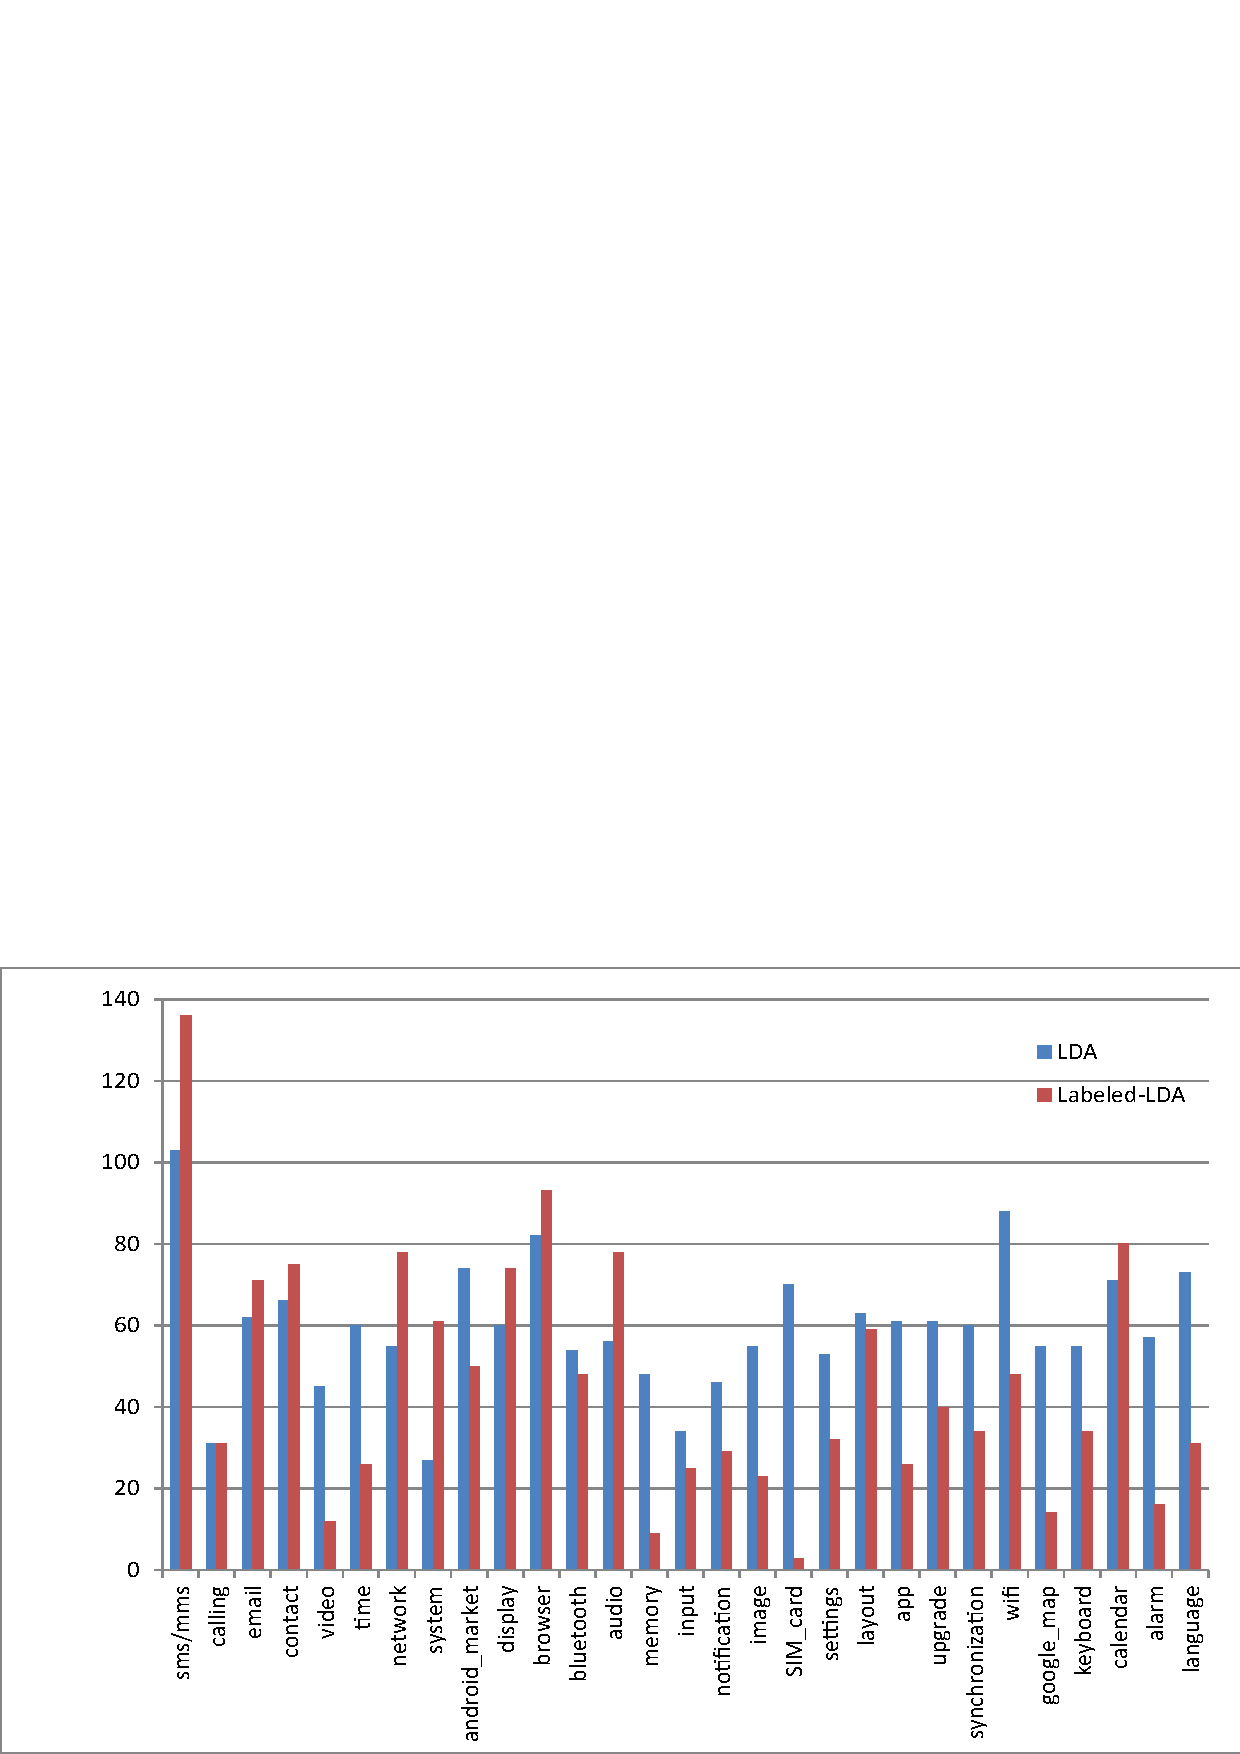
\includegraphics[width=0.4\textwidth]{htcldallda.png}
%\caption{Comparison of number of bug reports related to the same labels from LDA and Labeled LDA in HTC. The X axis is the same labels from LDA and Labeled-LDA and the Y axis is the number of bug reports.}
%\end{figure}
%
%\begin{figure}[htb]
%\centering
%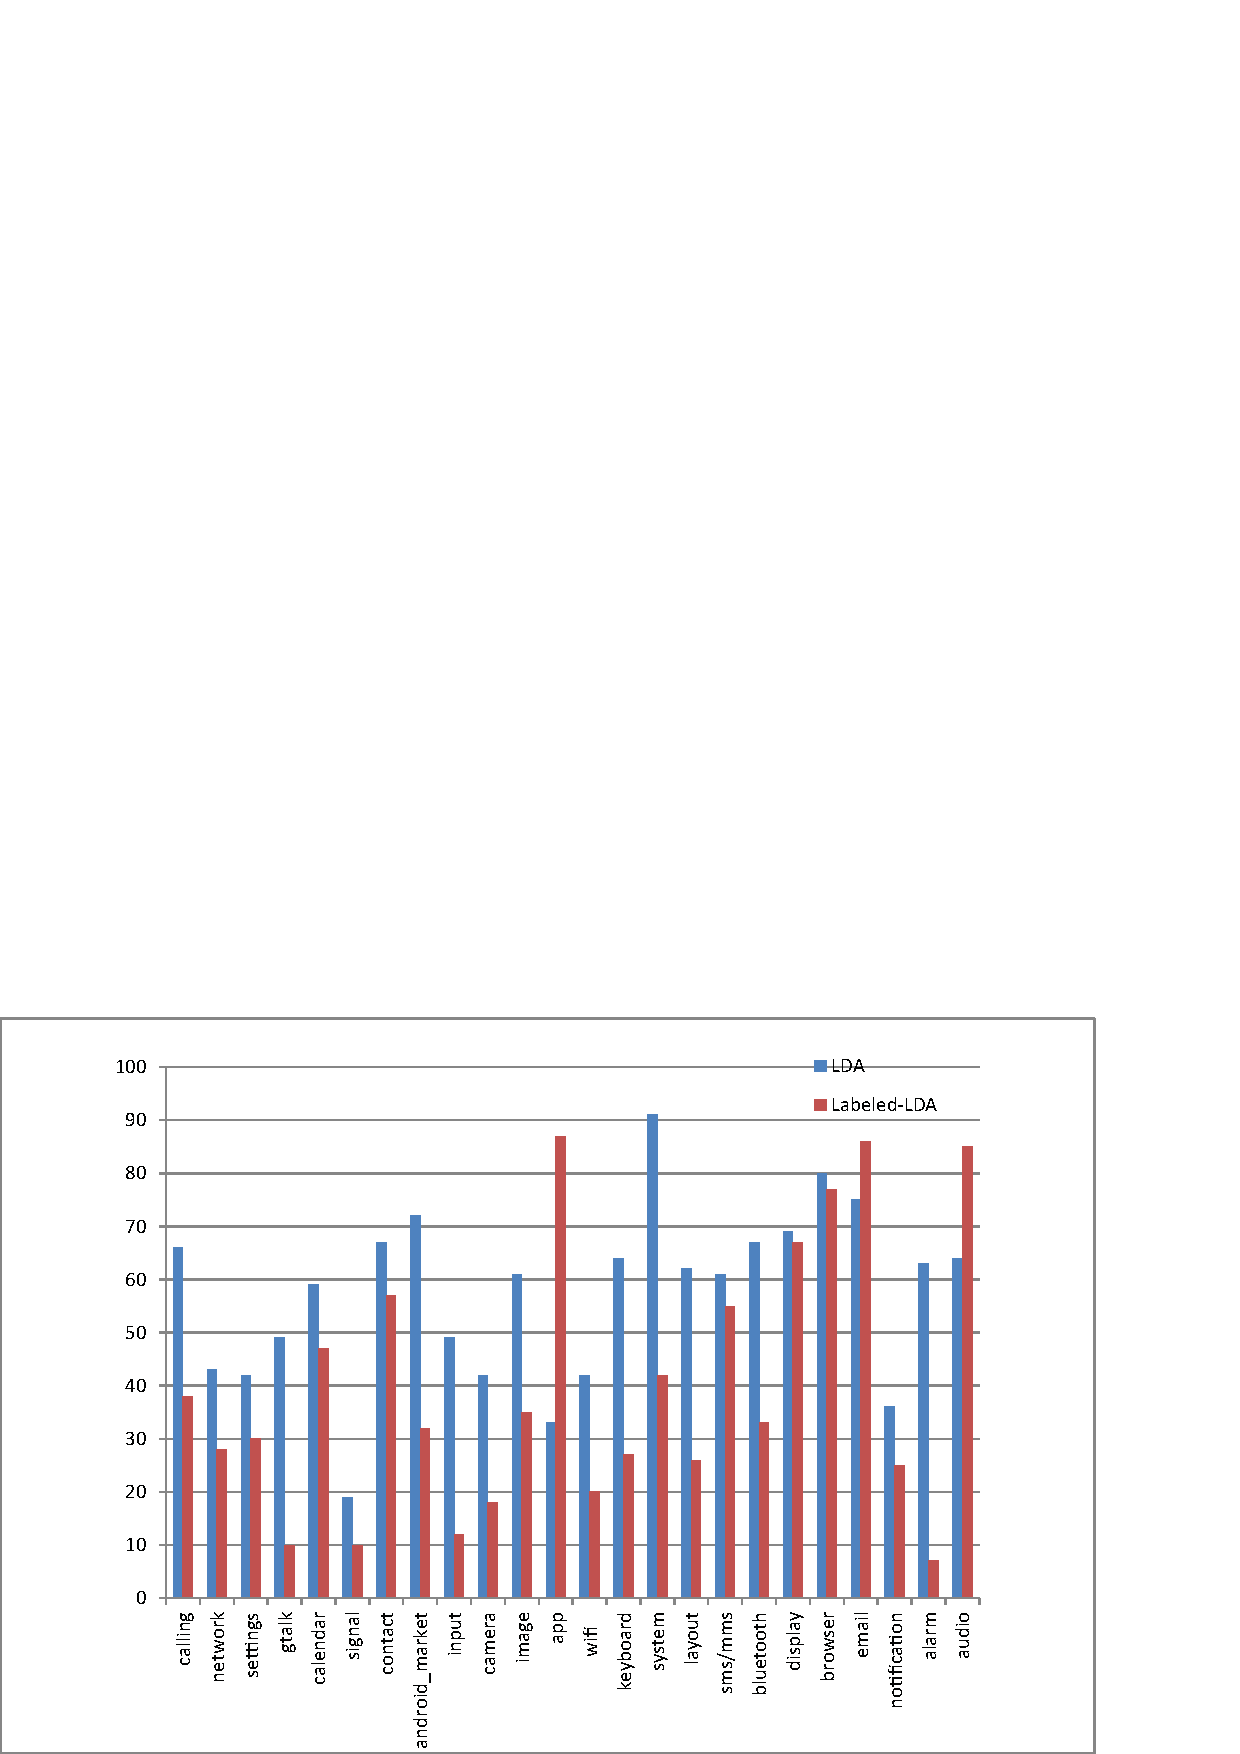
\includegraphics[width=0.4\textwidth]{motoldallda.png}
%\caption{Comparison of number of bug reports related to the same labels from LDA and Labeled-LDA in Motorola. The X axis is the same labels from LDA and Labeled-LDA and the Y axis is the number of bug reports.}
%\end{figure}
%
%\begin{figure}[htb]
%\centering
%\includegraphics[width=0.4\textwidth]{htcratiosim.png}
%\caption{The comparison of ratio and similarity in HTC. The result of the smaller number of bug reports related to this label in LDA or Labeled-LDA divided by the larger one is the ratio of this label. The X axis is the same labels from LDA and Labeled-LDA.}
%\end{figure}
%
%\begin{figure}[htb]
%\centering
%\includegraphics[width=0.4\textwidth]{motoratiosim.png}
%\caption{The comparison of ratio and similarity in Motorola. The result of the smaller number of bug reports related to this label in LDA or Labeled-LDA divided by the larger one is the ratio of this label. The X axis is the same labels from LDA and Labeled-LDA.}
%\end{figure}

% An example of a floating figure using the graphicx package.
% Note that \label must occur AFTER (or within) \caption.
% For figures, \caption should occur after the \includegraphics.
% Note that IEEEtran v1.7 and later has special internal code that
% is designed to preserve the operation of \label within \caption
% even when the captionsoff option is in effect. However, because
% of issues like this, it may be the safest practice to put all your
% \label just after \caption rather than within \caption{}.
%
% Reminder: the "draftcls" or "draftclsnofoot", not "draft", class
% option should be used if it is desired that the figures are to be
% displayed while in draft mode.
%
%\begin{figure}[!t]
%\centering
%\includegraphics[width=2.5in]{myfigure}
% where an .eps filename suffix will be assumed under latex, 
% and a .pdf suffix will be assumed for pdflatex; or what has been declared
% via \DeclareGraphicsExtensions.
%\caption{Simulation Results}
%\label{fig_sim}
%\end{figure}

% Note that IEEE typically puts floats only at the top, even when this
% results in a large percentage of a column being occupied by floats.


% An example of a double column floating figure using two subfigures.
% (The subfig.sty package must be loaded for this to work.)
% The subfigure \label commands are set within each subfloat command, the
% \label for the overall figure must come after \caption.
% \hfil must be used as a separator to get equal spacing.
% The subfigure.sty package works much the same way, except \subfigure is
% used instead of \subfloat.
%
%\begin{figure*}[!t]
%\centerline{\subfloat[Case I]\includegraphics[width=2.5in]{subfigcase1}%
%\label{fig_first_case}}
%\hfil
%\subfloat[Case II]{\includegraphics[width=2.5in]{subfigcase2}%
%\label{fig_second_case}}}
%\caption{Simulation results}
%\label{fig_sim}
%\end{figure*}
%
% Note that often IEEE papers with subfigures do not employ subfigure
% captions (using the optional argument to \subfloat), but instead will
% reference/describe all of them (a), (b), etc., within the main caption.


% An example of a floating table. Note that, for IEEE style tables, the 
% \caption command should come BEFORE the table. Table text will default to
% \footnotesize as IEEE normally uses this smaller font for tables.
% The \label must come after \caption as always.
%
%\begin{table}[!t]
%% increase table row spacing, adjust to taste
%\renewcommand{\arraystretch}{1.3}
%% if using array.sty, it might be a good idea to tweak the value of
%% \extrarowheight as needed to properly center the text within the cells
%\caption{An Example of a Table}
%\label{table_example}
%\centering
%% Some packages, such as MDW tools, offer better commands for making tables
%% than the plain LaTeX2e tabular which is used here.
%\begin{tabular}{|c||c|}
%\hline
%One & Two\\
%\hline
%Three & Four\\
%\hline
%\end{tabular}
%\end{table}


% Note that IEEE does not put floats in the very first column - or typically
% anywhere on the first page for that matter. Also, in-text middle ("here")
% positioning is not used. Most IEEE journals/conferences use top floats
% exclusively. Note that, LaTeX2e, unlike IEEE journals/conferences, places
% footnotes above bottom floats. This can be corrected via the \fnbelowfloat
% command of the stfloats package.


% use section* for acknowledgement
%\section*{Acknowledgment}


% trigger a \newpage just before the given reference
% number - used to balance the columns on the last page
% adjust value as needed - may need to be readjusted if
% the document is modified later
%\IEEEtriggeratref{8}
% The "triggered" command can be changed if desired:
%\IEEEtriggercmd{\enlargethispage{-5in}}

% Better way for balancing the last page:

%\balance

% references section

% can use a bibliography generated by BibTeX as a .bbl file
% BibTeX documentation can be easily obtained at:
% http://www.ctan.org/tex-archive/biblio/bibtex/contrib/doc/
% The IEEEtran BibTeX style support page is at:
% http://www.michaelshell.org/tex/ieeetran/bibtex/
%\bibliographystyle{IEEEtran}
% argument is your BibTeX string definitions and bibliography database(s)
%\bibliography{IEEEabrv,../bib/paper}
%
% <OR> manually copy in the resultant .bbl file
% set second argument of \begin to the number of references
% (used to reserve space for the reference number labels box)
%\begin{thebibliography}{1}

\def\IEEEbibitemsep{0pt plus .5pt}
\small
\bibliographystyle{IEEEtran}
\bibliography{IEEEabrv,msrreference}
%\bibliography{msrreference}




\end{document}
